% !TEX TS-program = xelatex
% !BIB program = bibtex
% !TeX spellcheck = ru_RU

% About magic macroses see also
% https://tex.stackexchange.com/questions/78101/

% По умолчанию используется шрифт 14 размера. Если нужен 12-й шрифт, уберите опцию [14pt]
\documentclass[14pt
  , russian
  %, xcolor={svgnames}
  ]{matmex-diploma-custom}
\usepackage[table]{xcolor}
\usepackage{graphicx}
\usepackage{tabularx}
\newcolumntype{Y}{>{\centering\arraybackslash}X}
\usepackage{amsmath}
\usepackage{amsthm}
\usepackage{amsfonts}
\usepackage{amssymb}
\usepackage{mathtools}
\usepackage{thmtools}
\usepackage{thm-restate}
\usepackage{tikz}
\usepackage{wrapfig}
% \usepackage[kpsewhich,newfloat]{minted}
% \usemintedstyle{vs}
\usepackage[inline]{enumitem}
\usepackage{subcaption}
\usepackage{caption}
%\usepackage[nocompress]{cite}
\usepackage{makecell}
% \setitemize{noitemsep,topsep=0pt,parsep=0pt,partopsep=0pt}
% \setenumerate{noitemsep,topsep=0pt,parsep=0pt,partopsep=0pt}


\graphicspath{ {resources/} }

%
% % \documentclass
% %   [ a4paper        % (Predefined, but who knows...)
% %   , draft,         % Show bad things.
% %   , 12pt           % Font size.
% %   , pagesize,      % Writes the paper size at special areas in DVI or
% %                    % PDF file. Recommended for use.
% %   , parskip=half   % Paragraphs: noindent + gap.
% %   , numbers=enddot % Pointed numbers.
% %   , BCOR=5mm       % Binding size correction.
% %   , submission
% %   , copyright
% %   , creativecommons
% %   ]{eptcs}
% % \providecommand{\event}{ML 2018}  % Name of the event you are submitting to
% % \usepackage{breakurl}             % Not needed if you use pdflatex only.
%
% \usepackage{underscore}           % Only needed if you use pdflatex.
%
% \usepackage{booktabs}
% \usepackage{amssymb}
% \usepackage{amsmath}
% \usepackage{mathrsfs}
% \usepackage{mathtools}
% \usepackage{multirow}
% \usepackage{indentfirst}
% \usepackage{verbatim}
% \usepackage{amsmath, amssymb}
% \usepackage{graphicx}
% \usepackage{xcolor}
% \usepackage{url}
% \usepackage{stmaryrd}
% \usepackage{xspace}
% \usepackage{comment}
% \usepackage{wrapfig}
% \usepackage[caption=false]{subfig}
% \usepackage{placeins}
% \usepackage{tabularx}
% \usepackage{ragged2e}
% \usepackage{soul}
\usepackage{csquotes}
% \usepackage{inconsolata}
%
% \usepackage{polyglossia}   % Babel replacement for XeTeX
%   \setdefaultlanguage[spelling=modern]{russian}
%   \setotherlanguage{english}
% \usepackage{fontspec}    % Provides an automatic and unified interface
%                          % for loading fonts.
% \usepackage{xunicode}    % Generate Unicode chars from accented glyphs.
% \usepackage{xltxtra}     % "Extras" for LaTeX users of XeTeX.
% \usepackage{xecyr}       % Help with Russian.
%
% %% Fonts
% \defaultfontfeatures{Mapping=tex-text}
% \setmainfont{CMU Serif}
% \setsansfont{CMU Sans Serif}
% \setmonofont{CMU Typewriter Text}

\usepackage[final]{listings}

\lstdefinelanguage{ocaml}{
keywords={@type, function, fun, let, in, match, with, when, class, type,
nonrec, object, method, of, rec, repeat, until, while, not, do, done, as, val, inherit, and,
new, module, sig, deriving, datatype, struct, if, then, else, open, private, virtual, include, success, failure,
lazy, assert, true, false, end},
sensitive=true,
commentstyle=\small\itshape\ttfamily,
keywordstyle=\ttfamily\bfseries, %\underbar,
identifierstyle=\ttfamily,
basewidth={0.5em,0.5em},
columns=fixed,
fontadjust=true,
literate={->}{{$\to$}}3 {===}{{$\equiv$}}1 {=/=}{{$\not\equiv$}}1 {|>}{{$\triangleright$}}3 {\\/}{{$\vee$}}2 {/\\}{{$\wedge$}}2 {>=}{{$\ge$}}1 {<=}{{$\le$}} 1,
morecomment=[s]{(*}{*)}
}

\lstset{
mathescape=true,
%basicstyle=\small,
identifierstyle=\ttfamily,
keywordstyle=\bfseries,
commentstyle=\scriptsize\rmfamily,
basewidth={0.5em,0.5em},
fontadjust=true,
language=ocaml
}

% перевод заголовков в листингах
\renewcommand\lstlistingname{Листинг}
\renewcommand\lstlistlistingname{Листинги}

\usepackage{caption}

% Add indent for listing captions
\DeclareCaptionFormat{listing}{
  %\parbox{\textwidth}{
    \hspace{15pt}#1#2#3
    %}
}
\captionsetup[lstlisting]{
  format=listing
  %, labelfont=white, textfont=white
  %  , singlelinecheck=false
  , margin=0pt
  , font={bf}
}

\usepackage[useregional]{datetime2}


\newcolumntype{L}[1]{>{\raggedright\let\newline\\\arraybackslash\hspace{0pt}}m{#1}}
\newcolumntype{C}[1]{>{\centering\let\newline\\\arraybackslash\hspace{0pt}}m{#1}}
\newcolumntype{R}[1]{>{\raggedleft\let\newline\\\arraybackslash\hspace{0pt}}m{#1}}



\usepackage{soul}
\usepackage[normalem]{ulem}
%\sout{Hello World}



\usepackage{afterpage}
\usepackage{pdflscape}

% swapping \phi and \varphi
% https://tex.stackexchange.com/a/50365/171947
\expandafter\mathchardef\expandafter\varphi\number\expandafter\phi\expandafter\relax
\expandafter\mathchardef\expandafter\phi\number\varphi

%https://tex.stackexchange.com/questions/30720/footnote-without-a-marker
\newcommand\blfootnote[1]{%
	\begingroup
	\renewcommand\thefootnote{}\footnote{#1}%
	\addtocounter{footnote}{-1}%
	\endgroup
}


% TODO: Понять, почему я выделил то, что тут в отдельный файл
\usepackage{listings}
\usepackage{tikz}
\usetikzlibrary{decorations.pathreplacing,calc,shapes,positioning,tikzmark}

\newcounter{tmkcount}

\tikzset{
  use tikzmark/.style={
    remember picture,
    overlay,
    execute at end picture={
      \stepcounter{tmkcount}
    },
  },
  tikzmark suffix={-\thetmkcount}
}


\usepackage{comment}
\usepackage{booktabs}%midrule/toprule/...

\usepackage{siunitx} % для таблиц с едлиницами измерений
\newcommand{\cd}[1]{\texttt{#1}}
\newcommand{\inbr}[1]{\left<#1\right>}

\newcommand{\OCaml}{\textsc{OCaml}}
\newcommand{\miniKanren}{\textsc{miniKanren}}
\newcommand{\BibTeX}{\textsc{BibTeX}}
\newcommand{\vsharp}{\textsc{V$\sharp$}}
\newcommand{\fsharp}{\textsc{F$\sharp$}}
\newcommand{\csharp}{\textsc{C$\sharp$}}
\newcommand{\GitHub}{\textsc{GitHub}}
\newcommand{\SMT}{\textsc{SMT}}


% Dependencies
\usepackage{totcount}
\usepackage{algorithm}% http://ctan.org/pkg/algorithms
\usepackage[noend]{algpseudocode}% http://ctan.org/pkg/algorithmicx
\usepackage{multirow}
\usepackage{nicematrix}
\usepackage{tikz}
\usetikzlibrary{fit}
\usetikzlibrary{arrows,automata}

% Custom
\theoremstyle{definition}
\newtheorem{rudefinition}{Определение}[section]
\newtheorem{example}{Example}[section]
\newtheorem{theorem}{Theorem}[section]
\newtheorem{proposition}[theorem]{Proposition}
\newtheorem{lemma}[theorem]{Lemma}
\newtheorem{corollary}[theorem]{Corollary}
\newtheorem{conjecture}[theorem]{Conjecture}
\newtheorem{note}[theorem]{Утверждение}
\newfontfamily{\cyrillicfonttt}{Liberation Mono}


\begin{document}

% Титульный лист (ГОСТ Р 7.0.11-2001, 5.1)
\thispagestyle{empty}
\begin{center}
\thesisOrganization
\end{center}
%
\vspace{0pt plus4fill} %число перед fill = кратность относительно некоторого расстояния fill, кусками которого заполнены пустые места
\IfFileExists{images/SPbGU_Logo.png}{
  \begin{minipage}[b]{0.5\linewidth}
    \begin{flushleft}
      %
\includegraphics[height=3.5cm]{SPbGU_Logo}
    \end{flushleft}
  \end{minipage}%
  \begin{minipage}[b]{0.5\linewidth}
    \begin{flushright}
      \underline{\textit{On the rights of the manuscript}}\\
%      \textsl {УДК \thesisUdk}
    \end{flushright}
  \end{minipage}
}{
\begin{flushright}
%Published as a manuscript
\underline{\textit{On the rights of the manuscript}}

%\textsl {УДК \thesisUdk}
\end{flushright}
}
%
\vspace{0pt plus6fill} %число перед fill = кратность относительно некоторого расстояния fill, кусками которого заполнены пустые места
\begin{center}
{\large \thesisAuthor}
\end{center}
%
\vspace{0pt plus1fill} %число перед fill = кратность относительно некоторого расстояния fill, кусками которого заполнены пустые места
\begin{center}
\textbf {\large %\MakeUppercase
\thesisTitle}

\vspace{0pt plus2fill} %число перед fill = кратность относительно некоторого расстояния fill, кусками которого заполнены пустые места

Scientific specialty

2.3.5. Mathematical and software support

for computers, complexes and computer networks

\vspace{0pt plus3fill} %число перед fill = кратность относительно некоторого расстояния fill, кусками которого заполнены пустые места

DISSERTATION

for the degree of Сandidate of Sciences in Physics and Mathematics

%
\vspace{0pt plus3fill}

Translation from Russian
\end{center}
\vspace{0pt plus4fill} %число перед fill = кратность относительно некоторого расстояния fill, кусками которого заполнены пустые места
\begin{flushright}
\ifdefined\supervisorTwoFio
Scientific supervisors:

\supervisorRegalia

\ifdefined\supervisorDead
\framebox{\supervisorFio}
\else
\supervisorFio
\fi

\supervisorTwoRegalia

\ifdefined\supervisorTwoDead
\framebox{\supervisorTwoFio}
\else
\supervisorFio
\fi
\else
Scientific supervisor:

\supervisorRegalia

\ifdefined\supervisorDead
\framebox{\supervisorFio}
\else
\supervisorFio
\fi
\fi

\end{flushright}
%
\vspace{0pt plus4fill} %число перед fill = кратность относительно некоторого расстояния fill, кусками которого заполнены пустые места
{\centering\thesisCity\

\thesisYear\par}

\maketitle
\setcounter{tocdepth}{2}
\tableofcontents

\section*{Введение}
% !TeX spellcheck = ru_RU
% !TEX root = vkr.tex

Современные компьютерные архитектуры позволяют легко обрабатывать линейные и иерархические структуры данных, такие как списки, стеки и деревья. Однако часто модель хранения данных представлена в виде графа. Такое представление применяется во множестве сфер: анализе социальных сетей, семантических сетей, анализе потока управления программ, биоинформатике и многих других.

Задача обработки данных, которые представлены в виде графа, имеет неструктурированный характер. Несмотря на это, некоторые алгоритмы анализа графов можно преобразовать к последовательности матрично-векторных операций, представив граф в виде матрицы смежности. Это позволяет выразить алгоритмы в терминах линейной алгебры, благодаря чему на практике за счет лучшего распараллеливания задачи удается получить эффективные реализации этих алгоритмов.

Более того, матрица смежности может быть представлена в разреженном виде, что позволяет сократить объем используемой памяти, так как в матрице хранятся только ненулевые элементы. Библиотеки разреженной линейной алгебры позволяют удобно работать с таким представлением. Они предоставляют набор примитивных операций таких, как матричное умножение, сложение, транспонирование, умножение вектора на матрицу и других, для работы с данными в разреженном виде.

Большую популярность в этом направлении набирает \verb|GraphBLAS|~\cite{intro_graphblas} --- стандарт, описывающий набор примитивных операций над матрицами и векторами, которые необходимы для выражения алгоритмов анализа графов в терминах линейной алгебры~\cite{intro_graphlastd}. Существует несколько реализаций этого стандарта, как, например, \verb|SuiteSparse:GraphBLAS|~\cite{intro_suitesparse}, которые удобно использовать для создания высокоэффективных алгоритмов анализа графов.

Одни из таких алгоритмов --- алгоритмы поиска путей в графе. В частности, в терминах линейной алгебры могут быть выражены алгоритмы поиска кратчайшего пути в графе, поиска путей между множеством начальных и конечных вершин. В случае, когда важно знать только о существовании пути между вершинами, говорят, что решают задачу достижимости в графе. При этом на множество искомых путей в графе могут накладываться дополнительные ограничения с помощью формальных языков. Для этого требуют, чтобы метки на ребрах искомого пути при конкатенации образовывали слова, принадлежащие заданному над некоторым алфавитом формальному языку.

Для создания ограничений используют регулярные и контекстно--свободные языки. Регулярные ограничения на пути в графе были впервые введены в работах~\cite{intro_rpq_term_appear1, intro_rpq_term_appear2} и нашли широкое применение в языках запросов к графовым базам данных~\cite{intro_rpq_massive_graphs}, которые позволяют эффективно хранить и обрабатывать связанные данные, такие как социальные сети, сети транспорта и многое другое. Контекстно--свободные языки позволяют выразить более широкий класс ограничений и используются также в областях статического анализа кода~\cite{intro_cfpq_code_analysis}, биоинформатике~\cite{intro_cfpq_bioinformatics} и других.

Запросы с регулярными ограничениями (RPQ) являются хорошо изучеными. Тем не менее в работе~\cite{intro_rpq_ineffective} было исследовано два подхода к решению задачи RPQ в языке запросов к графовым базам данных \verb|SPARQL|~\cite{intro_sparql}. Авторы работы выявили, что каждый из этих подходов эффективен только для конкретных видов графов.

В рамках учебной практики третьего курса автором данной работы был предложен новый алгоритм для решения задачи RPQ от множества стартовых вершин. Он был разработан на основе алгоритма поиска в ширину и реализован через примитивные операции разреженной линейной алгебры с помощью GraphBLAS. Для полученного алгоритма требуется провести экспериментальное исследование и сравнить его с аналогичными решениями.


\section{Постановка задачи}
% !TeX spellcheck = ru_RU
% !TEX root = vkr.tex

\label{sec:task}
Целью работы является проведение экспериментального исследования алгоритма для решения задачи RPQ, который нужно сравнить с аналогичными системами.

Для выполнения этой цели перед автором были поставлены следующие задачи.

\begin{itemize}
    \item  Выполнить обзор и выбрать множество инструментов, решающих задачу достижимости с регулярными ограничениями, для проведения сравнения с ними.
    \item  Подготовить набор данных, состоящий из графов и регулярных запросов, для проведения экспериментального исследования.
    \item Спроектировать инструмент для автоматизации экспериментов.
    \item Провести экспериментальное исследование и проанализировать его результаты.
\end{itemize}


\section{Обзор предметной области}
% !TeX spellcheck = ru_RU
% !TEX root = vkr.tex

\label{sec:relatedworks}
В данном разделе приводится терминология используемая в работе, представляются основные подходы для решения задачи поиска путей с регулярными ограничениями.

\subsection{Основы теории формальных языков}

В этой секции вводятся ключевые понятия из теории формальных языков, которые нужны для введения ограничений на пути в графе с помощью регулярных языков.

\begin{rudefinition} \emph{Формальной грамматикой} называется четверка \\ $\langle V_N, V_T, P, S \rangle$, где
    \begin{itemize}
        \item $V_N, V_T$ --- конечные и непересекающиеся алфавиты нетерминалов и терминалов соответственно;
        \item $P$ --- конечное множество правил;
        \item $S$ --- стартовый нетерминал.
    \end{itemize}
\end{rudefinition}

\begin{rudefinition} \emph{Праволинейной грамматикой} называется формальная грамматика, правила которой могут быть заданы как $A \rightarrow aB$, $A \rightarrow a$, $A \rightarrow \epsilon$.
\end{rudefinition}

\begin{rudefinition}
    \emph{Детерминированным конечным автоматом без эпсилон-переходов} называется пятерка $\langle Q, \Sigma, P, Q_{s}, F \rangle$, где
    \begin{itemize}
        \item $Q$ --- конечное непустое множество состояний;
        \item $\Sigma$ --- конечный входной алфавит;
        \item $P$ --- отображение $Q \times \Sigma \rightarrow Q$;
        \item $Q_{s} \subseteq Q$ --- множество начальных состояний;
        \item $F \subseteq Q$ --- множество конечных состояний.
    \end{itemize}
\end{rudefinition}

Далее, будем называть детерминированный конечный автомат без эпсилон-переходов --- конечным автоматом.

\begin{rudefinition} \emph{Регулярным выражением} над алфавитом $\Sigma$ называется
    \begin{itemize}
        \item $a$, если $a$ --- пустая строка, или $a \in \Sigma$;
        \item $e$ $\cdot$ $f$ (конкатенация), если $e$ и $f$ --- регулярные выражения;
        \item $e$ | $f$ (перечисление), если $e$ и $f$ --- регулярные выражения;
        \item $e^*$ (звезда Клини), если $e$ --- регулярное выражение.
    \end{itemize}
\end{rudefinition}

Для любого регулярного выражения существует представление в виде конечного автомата. Этот факт используется при построении алгоритмов, основанных на выражении регулярных ограничений с помощью конечных автоматов.

\subsection{Основные термины из теории графов}

\begin{rudefinition}\emph{Матрицей смежности} графа $\mathcal{G}$ называется матрица $M^{n \times n}$, где $n$ --- число вершин в графе, ячейка $M[i, j]$ имеет значение $l$, если существует ребро $e$ между вершинами $i$, $j$ с меткой $l$.
\end{rudefinition}

Заметим, что по каждой метке $l$ графа $\mathcal{G}$ можно построить матрицу смежности $\mathcal{M}^l$. Тогда ячейки матрицы $\mathcal{M}^l$ будут отражать факт наличия ребра $e$ с конкретной меткой $l$. Такое представление называется булевой декомпозицией матриц смежности графа. Оно позволяет хранить граф в виде набора булевых матриц, которыми удобно оперировать при построении алгоритмов на основе операций линейной алгебры.

Теперь можно сформулировать задачу поиска путей в графе с ограничениями, которые заданы с помощью регулярных языков. В частности, в данной работе рассматривается один из типов задачи поиска путей --- задача достижимости. Сформулируем эту задачу двумя способами. Они
отличаются в постановке результата, который ожидается в ходе решения задачи достижимости.

\begin{rudefinition} \emph{Задача достижимости с ограничениями в виде регулярных языков}. Пусть имеются:
    \begin{itemize}
        \item граф $\mathcal{G} = \langle V, E, L\rangle$;
        \item регулярный язык $\mathcal{L}$;
        \item множество стартовых $V_s \subseteq V$ и финальных $V_f \subseteq V$ вершин.
    \end{itemize}
    Рассмотрим пути $\pi = (v_0, e_0, \dots, e_n, v_n), e_k = (v_{k-1}, l_k, v_{k})$. Сопоставим каждому пути слово $W(\pi)=(l_0l_1 \dots l_{n-1}) \in \mathcal{L}$. Необходимо:

    \begin{itemize}
        \item Найти \textit{множество}, состоящее из вершин $v_n \in V$, для которых существует хотя бы один путь $\pi$ с началом в $v_0 \in V$ такой, что $W(\pi) \in \mathcal{L}$, $v_0 \in V_s$, $v_n \in V_f$.
        \item Найти все \textit{пары} вершин $v_0, v_n \in V$, для которых существует хотя бы один путь $\pi$ такой, что $W(\pi) \in \mathcal{L}$, $v_0 \in V_s$, $v_n \in V_f$.
    \end{itemize}
\end{rudefinition}

\subsection{Существующие решения}

В литературе выделяют несколько основных подходов к решению задачи поиска путей с ограничениями в виде регулярных языков. Они включают в себя подходы на основе конечных автоматов, использование программ на языке Datalog, построение индекса путей в графе для последующего исполнения регулярного запроса на основе индекса. Каждый из этих подходов будет подробнее рассмотрен в этой части обзора.

Алгоритмы для решения задачи PRQ на основе конечных автоматов строятся следующим образом. Входные данные в виде графа и регулярного языка представляются с помощью конечных автоматов. Для начала строится конечный автомат, который будет задавать регулярный язык. Далее, входной граф представляется в виде конечного автомата, у которого все состояния являются стартовыми и финальными. В итоге задачу поиска путей в графе с ограничениями, заданными с помощью регулярных языков, можно свести к задаче нахождения пересечения двух конечных автоматов.

Также вычислить пересечение конечных автоматов можно с использованием произведения Кронекера, которое применяется к матрицам из булевых декомпозиций матриц смежности для входного графа и представления конечного автомата в виде другого графа. Подробнее, использование матричных операций и произведения Кронекера рассматривается в разделе~\ref{2.4matr}.

\subsubsection{Подход с использованием языка Datalog}

Программа на Datalog представляет собой конечное множество правил. Правило --- это выражение следующей формы.

\begin{center}
    $h :$-- $p_1, p_2, \dots, p_n.$
\end{center}

Выражения $h, p_1, \dots, p_n$ представляют собой формулы вида \\$R(t_1, \dots, t_k)$, где $t_i$ может быть либо константой, либо переменной. Выражение $p_i$ --- факт, если все его $t_i$ являются константами.

    Для того, чтобы исполнять регулярные запросы с помощью программ на языке логического программирования Datalog, нужно представить граф в виде списка фактов о его ребрах.
    \begin{align*}
        edge(u_1 & ,l_1, v_1) \\
        edge(u_2 & ,l_2, v_2) \\
                 & \dots      \\
        edge(u_n & ,l_n, v_n)
    \end{align*}
    Где каждое ребро c меткой $l_i$, соединяет вершины $u_i$ $v_i$.

    Пример запроса $l^*$, который вычисляет транзитивное замыкание графа, содержащее рёбра с меткой $l$ можно описать следующим образом.

    \begin{center}
        $path(x, y) :$-- $edge(x, l, z), path(z, y).$\\
        $path(x, y) :$-- $edge(x, l, y).$
    \end{center}

    Имея представление запроса в виде регулярного выражения, можно получить программу на языке Datalog, которая будет исполнять этот запрос. Для этого нужно представить регулярное выражение с помощью правил грамматики, после чего транслировать грамматику во множество правил Datalog.

    Так, регулярное выражение $l^*$ может быть представлено правилами $S \rightarrow l$ $S$ и $S \rightarrow \epsilon$, которые легко транслируются в представленные выше правила Datalog.

Таким образом, для выполнения сравнения с этим подходом необходимо реализовать трансляцию регулярных выражений в программы на Datalog.

\subsubsection{Подход, основанный на построении индекса}

Существует множество работ на тему построения индекса путей в графе. Одни из них предлагают запоминать ключевые структуры в графе~\cite{related_frequent_fragments}, как, например, часто встречающиеся подграфы или другие фрагменты, описывающие основные свойства графа. Другой подход основан на индексировании путей и используется в работе~\cite{related_fletcher}, где авторы хранят пути размера не больше k, k --- целочисленная константа небольшого значения. Такой индекс позволяет исполнить любой регулярный запрос, состоящий не более чем из k меток, за один просмотр. Для запросов большего размера пути разделяются на части, длина которых кратна k, после чего запрос исполняется за несколько просмотров индекса.

Основным преимуществом построения индекса является то, что он позволяет быстро исполнить запрос по уже построенному пути. Однако использование индекса сказывается на размере потребляемой памяти во время работы алгоритма. Так, в исследовании~\cite{related_fletcher} самый большой граф имеет 131828 вершин, и для него авторы не смогли построить индекс, длина пути которого больше 2, в виду ограничений по памяти.

\subsection{Поиск путей с ограничениями с помощью операций над матрицами}\label{2.4matr}

Алгоритмы на основе матричных операций представляют еще один класс решений описанной задачи. Существует ряд алгоритмов, которые решают более общую задачу --- задачу КС-достижимости, однако они могут быть применены к регулярным ограничения на пути в том числе.

\subsubsection{Тензорный алгоритм}

Один из таких алгоритмов основан на произведении Кронекера~\cite{related_kron}. Он использует операции матричного умножения и не требует модификации изначальной контекстно-свободной грамматики.

На вход алгоритму подается конечный автомат, описывающий граф. Вторым аргументом алгоритм получает рекурсивный автомат, описывающий ограничения на пути в графе. Аналогично тому, как регулярное выражение может быть записано в виде конечного автомата, КС-грамматика может быть выражена с помощью рекурсивного автомата. Рекурсивный автомат может быть представлен в виде графа. Тогда, благодаря тензорному произведению, можно вычислить пересечение конечного автомата, соответствующего входному графу и рекурсивного автомата, соответствующего КС-ограничениям. После чего полученный автомат пересечения транзитивно замыкается. Эти операции применяются в цикле для булевой декомпозиции матриц смежности автомата, соответствующего КС-ограничениям, пока любая из матриц булевой декомпозиции меняется.

Операции вычисления транзитивного замыкания и тензорного произведения находят пути в графе для всех пар вершин. В случае, когда имеется множество стартовых вершин, производительность этого алгоритма может упасть, так как все вершины графа буду считаться начальными, и для всех них посчитаются пути до других вершин.


\section{Алгоритм, основанный на операциях линейной алгебры и поиске в ширину}
% !TeX spellcheck = ru_RU
% !TEX root = vkr.tex

В рамках учебной практики третьего курса автором был предложен новый алгоритм для решения задачи достижимости, основанный на классическом алгоритме поиска в ширину для нескольких стартовых вершин~\cite{method_msbfs}.

Идея алгоритма состоит в последовательном применении операции умножения матриц для совершения шага в алгоритме поиска в ширину. На примере~\ref{ex_graphblas} показано, как шаг в алгоритме поиска в ширину выражается с помощью операции умножения матрицы на вектор.

\begin{figure}[h!]
  \centering
  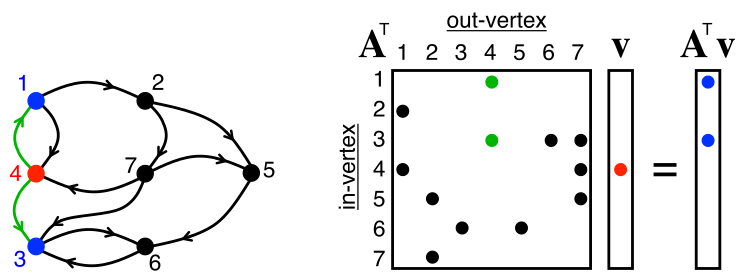
\includegraphics[width=0.7\linewidth]{pictures/AdjacencyMatrixGraphBLASBFS.png}
  \caption{Пример вычисления шага в алгоритме поиска в ширину, источник~\cite{method_gb_wiki}.}
\end{figure}\label{ex_graphblas}

Представленный далее алгоритм расширяет эту идею и применяет её для одновременного обхода графа и автомата, выражающего ограничения, заданные с помощью регулярного языка.

\subsection{Описание алгоритма}

Пусть дан граф $\mathcal{G} = \langle V, E, L\rangle$, регулярный язык, описывающий ограничения на пути в нем, и множество начальных вершин $V_{s}$ графа.
Известно, что регулярный язык может быть представлен с помощью детерминированного конечного автомата. Также известно, что конечный автомат может быть представлен с помощью графа с дополнительной информацией о стартовых и финальных состояниях. Представим полученный граф в виде матрицы смежности. Тогда регулярные ограничения могут быть выражены с помощью матрицы, ячейки которой описывают наличие перехода между двумя состояниями.  Более того, для задачи достижимости достаточно хранить в матрице смежности на $(i, j)$ месте два значения: $0$ --- отсутствие пути между вершинами $i$ и $j$, $1$ --- наличие пути.

Пусть каждой метке $l$ графа будет сопоставлена булева матрица смежности. Далее, будем оперировать с булевой декомпозицией матриц смежности $\mathcal{M}_A$ конечного автомата, и булевой декомпозицией матриц смежности $\mathcal{M}_G$ входного графа.

Алгоритм строит прямую сумму для матриц смежности $\mathcal{G}$ и $\mathcal{R}$. Представление в виде прямой суммы позволяет одновременно совершать шаг в алгоритме поиска в ширину на графе $\mathcal{G}$ и проверять удовлетворение регулярным ограничениям. Для каждого символа из пересечения множеств меток графа и алфавита регулярного языка построим матрицу $\mathcal{D} = \mathcal{M}_A \bigoplus \mathcal{M}_G$.

\begin{equation}
  \mathcal{D} =
  \left[
    \begin{matrix}
      \mathcal{M}_A & 0             \\
      0             & \mathcal{M}_G
    \end{matrix}
    \right]
\end{equation}

Далее, опишем процедуру обхода, основанную на серии умножений матрицы смежности.
В классической версии обхода используется вектор $v$, куда записывается фронт обхода графа. Так, один раз перемножая матрицу смежности на вектор $v$, можно совершать один шаг в обходе графа, как было показано в примере~\ref{ex_graphblas}.

Пусть $k$ --- количество вершин в графе, построенном по конечному автомату, $n$ --- количество вершин в графе $\mathcal{G}$. Тогда первые $k$ элементов вектора $v$ хранят информацию о номере состояния конечного автомата, построенного по $\mathcal{R}$, оставшиеся $n$ элементов хранят информацию о номере вершины входного графа. При этом для проверки путей на соответствие входным регулярным ограничениям необходимо иметь информацию о парах $(v_i, v_j)$, $0<= i < k, k <= j < k+n$. Каждая из этих пар хранит информацию о том, в каком состоянии $v_i$ мы оказались, достигнув вершину $v_j$. Предлагается разложить вектор $v$ во множество векторов $v^{0}, v^{1}, ... v^{k}$ и получить матрицу $M$ вида.

\begin{equation}
  M^{k \times (k + n)} =
  \left[
    \begin{matrix}
      v^{0} \\
      v^{1} \\
      \dots \\
      v^{k}
    \end{matrix}
    \right]
\end{equation}

Построенная таким образом матрица $M$ содержит информацию о достигнутых во время обхода вершинах графа. Остается лишь ограничить левую часть векторов $v^i$ таким образом, чтобы они всегда содержали только одну единицу, что позволит определить в каком состоянии вершина была достигнута. Для этого скажем, что $v^i[i] = 1$, $v^i[j] = 0$ при $i \neq j$. Тогда $v^i$ будет соответствовать $i$ номеру состояния $\mathcal{R}$, и правая часть вектора $v^i$ будет содержать информацию о достижимых вершинах. Матрица $M$ примет вид.

\begin{equation}
  M^{k \times (k + n)} =
  \left[
    \begin{matrix}
      Id_k & Matrix_{k \times n }
    \end{matrix}
    \right]
\end{equation}

Где $Id_k$ --- единичная матрица, $Matrix_{k \times n }$ --- матрица, хранящая фронт вершин в графе для каждого состояния.

В итоге остается проинициализировать множество начальных вершин. Для этого нужно, чтобы в ячейке $(i, i+j+1)$ матрицы $M$ стояла 1, если состояние конечного автомата, построенного по $\mathcal{R}$, соответствующее номеру $i$, является начальным, а вершина графа $\mathcal{G}$ соответствующая номеру $j$ содержится в множестве начальных вершин, то есть $j \in V_{s}$.

Перейдем к построению алгоритма, который представлен на листинге~\ref{BFSRPQ1}. На вход алгоритм принимает граф и ограничения в виде регулярного языка, которые можно представить с помощью конечного автомата.

Алгоритм обхода заключается в последовательном умножении матрицы $M$ текущего фронта на матрицу $\mathcal{D}$. В результате чего, получается матрица $M'$ содержащая информацию о вершинах, достижимых на следующем шаге. Далее, с помощью операций перестановки и сложения векторов $M'$ преобразуется к виду матрицы $M$ и присваивается ей для совершения нового шага.
Важно отметить, что на каждом шаге хранится матрица $M_{all}$, которая наполняется значениями, полученными на текущем шаге. Итерации продолжаются пока меняется $M_{all}$.

\begin{algorithm}[t]
  \caption{Алгоритм в терминах линейной алгебры
    для поиска путей от нескольких стартовых
    вершин с регулярными ограничениями}\label{BFSRPQ1}
  \begin{algorithmic}[1]
    \Procedure{MSBFS~} {$\mathcal{R}=\langle Q, \Sigma, P, F, Q_{s} \rangle,\mathcal{G}=\langle V, E, L \rangle, V_{s}$}

    \State $k\gets |Q|$, $n\gets |V|$
    \State $\mathcal{M}_A\gets $ булева декомпозиция матрицы смежности для $\mathcal{R}$
    \State $\mathcal{M}_G\gets $ булева декомпозиция матрицы смежности для $\mathcal{G}$

    \ForAll{$q\in Q_{s}$\label{init_m_1}}
    \ForAll{$v\in V_{s}$\label{init_m_2}}
    \State $M[q,q+v+1]\gets 1$ \Comment{Где $M^{k \times (k + n)}$ с 1 на главной диагонали\label{init_m_3}}
    \EndFor
    \EndFor

    \ForAll{$a\in (\Sigma \cap L)$}
    \State $\mathcal{D}_a\gets \mathcal{M}_A \bigoplus \mathcal{M}_G$
    \EndFor

    \State $M'\gets M$, $M_{all}\gets M$
    \While{Матрица~$M_{all}$~меняется}
    \State $M\gets M'\langle\neg M_{all}\rangle$
    \ForAll{$a\in (\Sigma \cap L)$}
    \State $M'\gets M~$any.pair$~\mathcal{D}_a$
    \Comment{Матр. умножение в полукольце}
    \State $M'\gets TransformRows(M')$\label{TransformRows}\Comment{Приведение $M'$ к виду $M$}
    \State $M_{all}\gets M'$
    \EndFor
    \EndWhile
    \State \textbf{return} $M_{all}$
    \EndProcedure
  \end{algorithmic}
\end{algorithm}

В алгоритме~\ref{BFSRPQ1} на~\ref{TransformRows} строке происходит трансформация строчек в матрице $M'$. Это делается для того, чтобы представить полученную во время обхода матрицу $M'$, содержащую новый фронт, в виде матрицы $M$ для совершения последующих шагов. Для этого требуется так переставить строчки $M'$, чтобы она содержала корректные по определению $M$ значения. То есть, имела единицы на главной диагонали, а все остальные значения в первых $k$ столбцах были нулями. Подробнее эта процедура описана в листинге~\ref{AlgoTransformRows}.

\begin{algorithm}[H]
  \caption{Алгоритм трансформации строчек}\label{AlgoTransformRows}
  \begin{algorithmic}[1]
    \Procedure{TransformRows}{$M$}
    \State{$T \gets extractLeftSubMatrix(M)$}
    \State{$Ix, Iy \gets$ итераторы по индексам ненулевых элементов $T$}
    \For{$i \in 0\dots|Iy|$}
    \State{$R\gets M.getRow(Ix[i])$}
    \State{$M'.setRow(Iy[i], R + M'.getRow(Iy[i]))$}
    \EndFor
    \EndProcedure
  \end{algorithmic}
\end{algorithm}

В итоге алгоритм~\ref{BFSRPQ1} решает задачу достижимости с регулярными ограничениями, так как матрица $M_{all}$ содержит всю необходимую информацию о достигнутых вершинах. Для всех вершин $f$, соответствующих конечным состояниям $F$ автомата, построенного по $\mathcal{R}$, в ячейке $M_{all}[f, f + i + 1]$ будет храниться единица, если вершина $i$ во входном графе достижима из множества начальных вершин. Результатом работы алгоритма является матрица $M_{all}$, которая хранит информацию о множестве достигнутых вершин.

\subsection{Пример}

Рассмотрим работу алгоритма, представленного на листинге~\ref{BFSRPQ1}, на примере. Пусть имеется граф.
\begin{center}
  \label{input_rpq}
  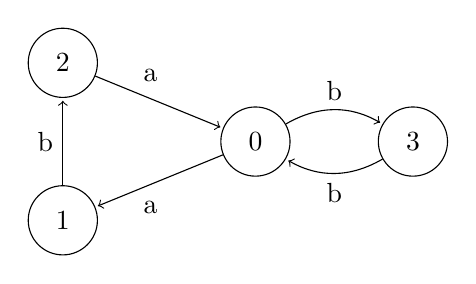
\begin{tikzpicture}[node distance=2cm,shorten >=1pt,on grid,auto]
    \node[state] (q_0)   {$1$};
    \node[state] (q_1) [above=of q_0] {$2$};
    \node[state] (q_2) [right=of $(q_0)!0.5!(q_1)$] {$0$};
    \node[state] (q_3) [right=of q_2] {$3$};
    \path[->]
    (q_0) edge  node {b} (q_1)
    (q_1) edge  node[pos=0.3] {a} (q_2)
    (q_2) edge  node[pos=0.7] {a} (q_0)
    (q_2) edge[bend left]  node[above] {b} (q_3)
    (q_3) edge[bend left]  node {b} (q_2);
  \end{tikzpicture}
\end{center}

Для него алгоритм инициализирует следующие матрицы: матрицу смежности $M_G$ и её булеву декомпозицию по каждой метке.
\[ M_G =
  \begin{pmatrix}
    .     & \{a\} & .     & \{b\} \\
    .     & .     & \{b\} & .     \\
    \{a\} & .     & .     & .     \\
    \{b\} & .     & .     & .
  \end{pmatrix}
\]

\begin{alignat}{7}
   &  &  & \mathcal{M}_{G\_a} &  & = \begin{pmatrix}
                                       0 & 1 & 0 & 0 \\
                                       0 & 0 & 0 & 0 \\
                                       1 & 0 & 0 & 0 \\
                                       0 & 0 & 0 & 0 \\
                                     \end{pmatrix} \ \ \ \  &  & \mathcal{M}_{G\_b} &  & = \begin{pmatrix}
                                                                                             0 & 0 & 0 & 1 \\
                                                                                             0 & 0 & 1 & 0 \\
                                                                                             0 & 0 & 0 & 0 \\
                                                                                             1 & 0 & 0 & 0 \\
                                                                                           \end{pmatrix}
\end{alignat}

Зададим ограничения с помощью регулярного выражения $b^*ab$, которое представляется автоматом из трех последовательных состояний.

\begin{center}
  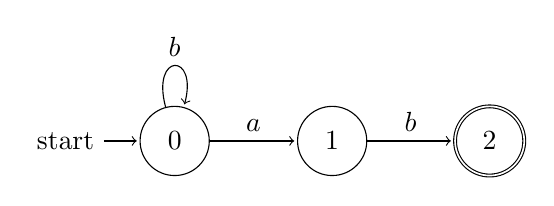
\begin{tikzpicture}[shorten >=1pt,on grid,auto]
    \node[state, initial]   (q_0) at (0,0)  {$0$};
    \node[state]             (q_1) at (2,0)  {$1$};
    \node[state, accepting] (q_2) at (4,0)  {$2$};
    \path[->]
    (q_0) edge  node {$a$} (q_1)
    (q_1) edge  node {$b$} (q_2);
    \draw (q_0) edge[loop above]  node {$b$} (q_0);
  \end{tikzpicture}
\end{center}


Автомат может быть задан матрицей смежности (с дополнительной информацией о стартовых и финальных состояниях). Для регулярного выражения $b^*ab$ булева декомпозиция матрицы смежности выглядит следующим образом (при этом нужно запомнить, что
состояние $0$ является начальным, $2$ --- конечным).

\[ M_A =
  \begin{pmatrix}
    \{b\} & \{a\} & .     \\
    .     & .     & \{b\} \\
    .     & .     & .
  \end{pmatrix}
\]

\begin{alignat}{7}
   &  &  & \mathcal{M}_{A\_a} &  & = \begin{pmatrix}
                                       0 & 1 & 0 \\
                                       0 & 0 & 0 \\
                                       0 & 0 & 0
                                     \end{pmatrix} \ \ \ \  &  & \mathcal{M}_{A\_b} &  & = \begin{pmatrix}
                                                                                             1 & 0 & 0 \\
                                                                                             0 & 0 & 1 \\
                                                                                             0 & 0 & 0
                                                                                           \end{pmatrix}
\end{alignat}

Для синхронизации обхода алгоритм в строчках 8--9 составляет набор блочно-диагональных матриц, каждая из которых --- это прямая сумма двух матриц булевой декомпозиции:
$\mathcal{D}_{a} = \mathcal{M}_{A\_a} \oplus \mathcal{M}_{G\_a}$ и $\mathcal{D}_{b} = \mathcal{M}_{A\_b} \oplus \mathcal{M}_{G\_b}$.

\begin{alignat}{7}
           &  &                 & \mathcal{D}_{a} &   & =
  \begin{pNiceArray}{ccc:cccc}
    0 & 1 & 0 & 0 & 0 & 0 & 0 \\
    0 & 0 & 0 & 0 & 0 & 0 & 0 \\
    0 & 0 & 0 & 0 & 0 & 0 & 0 \\
    \hdottedline
    0 & 0 & 0 & 0 & 1 & 0 & 0 \\
    0 & 0 & 0 & 0 & 0 & 0 & 0 \\
    0 & 0 & 0 & 1 & 0 & 0 & 0 \\
    0 & 0 & 0 & 0 & 0 & 0 & 0
    \CodeAfter
    \OverBrace[shorten,yshift=3pt]{1-1}{2-3}{automaton}
    \UnderBrace[shorten,yshift=3pt]{7-4}{7-7}{graph}
  \end{pNiceArray}
  \ \ \ \  &  & \mathcal{D}_{b} &                 & =
  \begin{pNiceArray}{ccc:cccc}
    1 & 0 & 0 & 0 & 0 & 0 & 0 \\
    0 & 0 & 1 & 0 & 0 & 0 & 0 \\
    0 & 0 & 0 & 0 & 0 & 0 & 0 \\
    \hdottedline
    0 & 0 & 0 & 0 & 0 & 0 & 1 \\
    0 & 0 & 0 & 0 & 0 & 1 & 0 \\
    0 & 0 & 0 & 0 & 0 & 0 & 0 \\
    0 & 0 & 0 & 1 & 0 & 0 & 0
    \CodeAfter
    \OverBrace[shorten,yshift=3pt]{1-1}{2-3}{automaton}
    \UnderBrace[shorten,yshift=3pt]{7-4}{7-7}{graph}
  \end{pNiceArray}
\end{alignat}\\

Пусть мы решаем частный случай задачи достижимости с несколькими стартовыми вершинами (multiple-source)
--- достижимость с одной стартовой вершиной (single-source). Пусть единственной начальной вершиной в графе будет вершина $0$.

В строчках 5--7  алгоритм инициализирует матрицу $M$. Для этого единицами заполняются ячейки на главной дианогали, а также те ячейки, которые соответствуют вершинам из множества стартовых.

\begin{alignat}{7}
   &  &  & M &  & =\begin{NiceMatrix}
                     \fbox{1 0 0} \fbox{1 0 0 0} \\
                     \fbox{0 1 0} \fbox{0 0 0 0} \\
                     \fbox{0 0 1} \fbox{0 0 0 0}
                   \end{NiceMatrix}
\end{alignat}

На первой итерации алгоритма происходит умножение матриц $M$ и $\mathcal{D}$ для совершения одного шага в обходе графа.

\begin{alignat}{7}
  a:\,\,
   & \begin{matrix}
       \fbox{1 0 0} \fbox{1 0 0 0} \\
       \fbox{0 1 0} \fbox{0 0 0 0} \\
       \fbox{0 0 1} \fbox{0 0 0 0}
     \end{matrix} &                                &
  \times
  \begin{pNiceArray}{ccc:cccc}
    0 & 1 & 0 & 0 & 0 & 0 & 0 \\
    0 & 0 & 0 & 0 & 0 & 0 & 0 \\
    0 & 0 & 0 & 0 & 0 & 0 & 0 \\
    \hdottedline
    0 & 0 & 0 & 0 & 1 & 0 & 0 \\
    0 & 0 & 0 & 0 & 0 & 0 & 0 \\
    0 & 0 & 0 & 1 & 0 & 0 & 0 \\
    0 & 0 & 0 & 0 & 0 & 0 & 0
  \end{pNiceArray}
   &                                & = \begin{NiceMatrix}
                                          \fbox{0 1 0} \fbox{0 1 0 0} \\
                                          \fbox{0 0 0} \fbox{0 0 0 0} \\
                                          \fbox{0 0 0} \fbox{0 0 0 0}
                                          \CodeAfter
                                          \begin{tikzpicture}
      \draw [thick,red] (2-1.west) -- (2-1.east) ;
      \draw [thick,red] (3-1.west) -- (3-1.east) ;
    \end{tikzpicture}
                                        \end{NiceMatrix}
\end{alignat}

\begin{alignat}{7}
  b:\,\,
   & \begin{matrix}
       \fbox{1 0 0} \fbox{1 0 0 0} \\
       \fbox{0 1 0} \fbox{0 0 0 0} \\
       \fbox{0 0 1} \fbox{0 0 0 0}
     \end{matrix} &                                &
  \times
  \begin{pNiceArray}{ccc:cccc}
    1 & 0 & 0 & 0 & 0 & 0 & 0 \\
    0 & 0 & 1 & 0 & 0 & 0 & 0 \\
    0 & 0 & 0 & 0 & 0 & 0 & 0 \\
    \hdottedline
    0 & 0 & 0 & 0 & 0 & 0 & 1 \\
    0 & 0 & 0 & 0 & 0 & 1 & 0 \\
    0 & 0 & 0 & 0 & 0 & 0 & 0 \\
    0 & 0 & 0 & 1 & 0 & 0 & 0
  \end{pNiceArray}
   &                                & = \begin{NiceMatrix}
                                          \fbox{1 0 0} \fbox{0 0 0 1} \\
                                          \fbox{0 0 1} \fbox{0 0 0 0} \\
                                          \fbox{0 0 0} \fbox{0 0 0 0}
                                          \CodeAfter
                                          \begin{tikzpicture}
      \draw [thick,red] (3-1.west) -- (3-1.east) ;
    \end{tikzpicture}
                                        \end{NiceMatrix}
\end{alignat}

Для того, чтобы левая часть матрицы $M$ всегда оставалась единичной, в строке 15 алгоритма происходит трансформация строчек матрицы $M'$, которая в итоге присваивается $M$ в строчке 12. Для этого происходит сложение тех строчек матрицы $M'$, у которых в левой части единицы стоят на одинаковых позициях. После чего в матрице $M'$ строчки переставляются так, чтобы левая часть $M'$ принимала единичный вид. Строчки с пустой левой частью при этом не рассматриваются. После этих трансформаций правая часть матрицы $M'$ кодирует фронт обхода графа для каждого состояния конечного автомата.

В нашем примере полученная матрица $M'$ для следующего шага обхода выглядит следующим образом. В матрицу $M_{all}$ при этом записывается накопленный результат.

\begin{alignat}{7}
   &  &  & M_{all} = M' &  & =\begin{matrix}
                                \fbox{1 0 0} \fbox{0 0 0 1} \\
                                \fbox{0 1 0} \fbox{0 1 0 0} \\
                                \fbox{0 0 1} \fbox{0 0 0 0}
                              \end{matrix}
\end{alignat}

Видно, что во фронт обхода графа попали вершины 1 и 3. В вершину 1 мы попали в состоянии 1, в вершину 3 --- в состоянии 0. Совершаются следующие переходы в графе и автомате.

\begin{alignat}{7}
  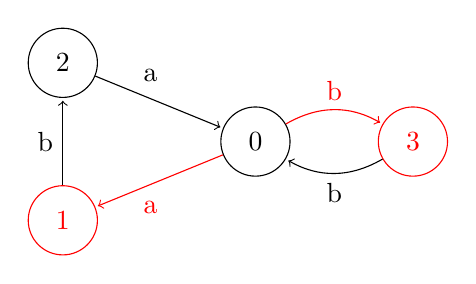
\begin{tikzpicture}[node distance=2cm,shorten >=1pt,on grid,auto]
    \node[state, red] (q_0)   {$1$};
    \node[state] (q_1) [above=of q_0] {$2$};
    \node[state] (q_2) [right=of $(q_0)!0.5!(q_1)$] {$0$};
    \node[state, red] (q_3) [right=of q_2] {$3$};
    \path[->, red]
    (q_2) edge  node[pos=0.7] {a} (q_0)
    (q_2) edge[bend left]  node[above] {b} (q_3);
    \path[->]
    (q_0) edge  node {b} (q_1)
    (q_1) edge  node[pos=0.3] {a} (q_2)
    (q_3) edge[bend left]  node {b} (q_2);
  \end{tikzpicture}
  \qquad
  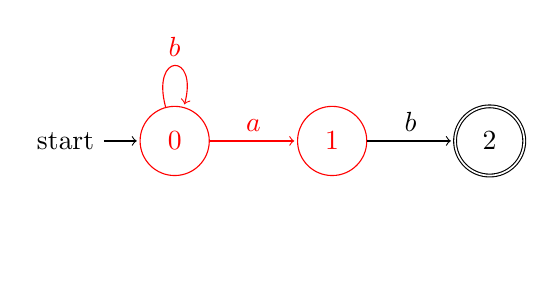
\begin{tikzpicture}[shorten >=1pt,on grid,auto]
    \node[state, draw=none]      (q_3) at (0,0)  {}; % empty node for alignment
    \node[state, initial, red]   (q_0) at (0,1)  {$0$};
    \node[state, red]            (q_1) at (2,1)  {$1$};
    \node[state, accepting]      (q_2) at (4,1)  {$2$};
    \path[->, red]
    (q_0) edge  node {$a$} (q_1);
    \path[->]
    (q_1) edge  node {$b$} (q_2);
    \draw (q_0) edge[loop above, red]  node {$b$} (q_0);
  \end{tikzpicture}
\end{alignat}

Совершим еще одну итерацию алгоритма.

\begin{alignat}{7}
  a:\,\,
   & \begin{matrix}
       \fbox{1 0 0} \fbox{0 0 0 1} \\
       \fbox{0 1 0} \fbox{0 1 0 0} \\
       \fbox{0 0 1} \fbox{0 0 0 0}
     \end{matrix} &                                &
  \times
  \begin{pNiceArray}{ccc:cccc}
    0 & 1 & 0 & 0 & 0 & 0 & 0 \\
    0 & 0 & 0 & 0 & 0 & 0 & 0 \\
    0 & 0 & 0 & 0 & 0 & 0 & 0 \\
    \hdottedline
    0 & 0 & 0 & 0 & 1 & 0 & 0 \\
    0 & 0 & 0 & 0 & 0 & 0 & 0 \\
    0 & 0 & 0 & 1 & 0 & 0 & 0 \\
    0 & 0 & 0 & 0 & 0 & 0 & 0
  \end{pNiceArray}
   &                                & = \begin{NiceMatrix}
                                          \fbox{0 1 0} \fbox{0 0 0 0} \\
                                          \fbox{0 0 0} \fbox{0 0 0 0} \\
                                          \fbox{0 0 0} \fbox{0 0 0 0}
                                          \CodeAfter
                                          \begin{tikzpicture}
      \draw [thick,red] (2-1.west) -- (2-1.east) ;
      \draw [thick,red] (3-1.west) -- (3-1.east) ;
    \end{tikzpicture}
                                        \end{NiceMatrix}
\end{alignat}

\begin{alignat}{7}
  b:\,\,
   & \begin{matrix}
       \fbox{1 0 0} \fbox{0 0 0 1} \\
       \fbox{0 1 0} \fbox{0 1 0 0} \\
       \fbox{0 0 1} \fbox{0 0 0 0}
     \end{matrix} &                                &
  \times
  \begin{pNiceArray}{ccc:cccc}
    1 & 0 & 0 & 0 & 0 & 0 & 0 \\
    0 & 0 & 1 & 0 & 0 & 0 & 0 \\
    0 & 0 & 0 & 0 & 0 & 0 & 0 \\
    \hdottedline
    0 & 0 & 0 & 0 & 0 & 0 & 1 \\
    0 & 0 & 0 & 0 & 0 & 1 & 0 \\
    0 & 0 & 0 & 0 & 0 & 0 & 0 \\
    0 & 0 & 0 & 1 & 0 & 0 & 0
  \end{pNiceArray}
   &                                & = \begin{NiceMatrix}
                                          \fbox{1 0 0} \fbox{1 0 0 0} \\
                                          \fbox{0 0 1} \fbox{0 0 1 0} \\
                                          \fbox{0 0 0} \fbox{0 0 0 0}
                                          \CodeAfter
                                          \begin{tikzpicture}
      \draw [thick,red] (3-1.west) -- (3-1.east) ;
    \end{tikzpicture}
                                        \end{NiceMatrix}
\end{alignat}

\tikzset{highlight/.style={rectangle,
      fill=teal!15,
      rounded corners = 0.5 mm,
      inner sep=1pt,
      fit=#1}}

\begin{alignat}{7}
   &          &  & M'      &  & =\begin{NiceMatrix}
                                   \fbox{1 0 0} \fbox{1 0 0 0} \\
                                   \fbox{0 1 0} \fbox{0 0 0 0} \\
                                   \fbox{0 0 1} \fbox{0 0 1 0}
                                   \CodeAfter
                                 \end{NiceMatrix}
   & \ \ \ \
   &          &  & M_{all} &  & =\begin{NiceMatrix}
                                   \CodeBefore [create-cell-nodes]
                                   \tikz \node(3-1) {} [highlight = (3-1)] {} ;
                                   \Body
                                   \fbox{1 0 0} \fbox{1 0 0 1} \\
                                   \fbox{0 1 0} \fbox{0 1 0 0} \\
                                   \fbox{0 0 1} \fbox{0 0 1 0}
                                 \end{NiceMatrix}
\end{alignat}

\begin{alignat}{7}
  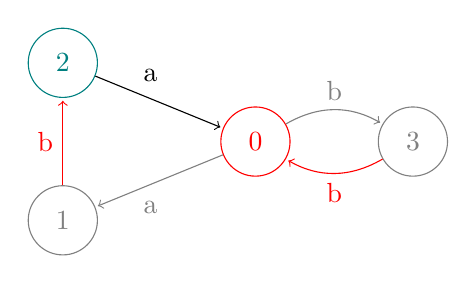
\begin{tikzpicture}[node distance=2cm,shorten >=1pt,on grid,auto]
    \node[state, gray] (q_0)   {$1$};
    \node[state, teal] (q_1) [above=of q_0] {$2$};
    \node[state, red] (q_2) [right=of $(q_0)!0.5!(q_1)$] {$0$};
    \node[state, gray] (q_3) [right=of q_2] {$3$};
    \path[->, gray]
    (q_2) edge  node[pos=0.7] {a} (q_0)
    (q_2) edge[bend left]  node[above] {b} (q_3);
    \path[->, red]
    (q_0) edge  node {b} (q_1)
    (q_3) edge[bend left]  node {b} (q_2);
    \path[->]
    (q_1) edge  node[pos=0.3] {a} (q_2);
  \end{tikzpicture}
  \qquad
  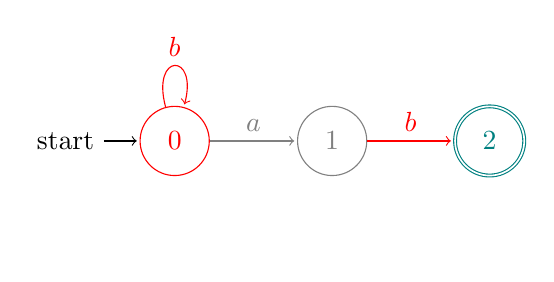
\begin{tikzpicture}[shorten >=1pt,on grid,auto]
    \node[state, draw=none]            (q_3) at (0,0)  {}; % empty node for alignment
    \node[state, initial, red]         (q_0) at (0,1)  {$0$};
    \node[state, gray]                 (q_1) at (2,1)  {$1$};
    \node[state, accepting, teal]      (q_2) at (4,1)  {$2$};
    \path[->, gray]
    (q_0) edge  node {$a$} (q_1);
    \path[->, red]
    (q_1) edge  node {$b$} (q_2);
    \draw (q_0) edge[loop above, red]  node {$b$} (q_0);
  \end{tikzpicture}
\end{alignat}

Видно, что мы достигли вершины 2 графа в конечном состоянии 2 автомата. При этом вершины графа 0, 1, 3 также достигнуты, однако это происходит в состояниях автомата 0, 1, 0 соответственно, которые не являются конечными.

Результатом работы алгоритма является матрица $M_{all}$, в которой содержится вся необходимая информация о достигнутых вершинах. В частности, для конечного состояния 2: $M_{all}[2, 5]$ = 1 означает, что мы получили множество достижимых вершин, состоящее из одной вершины 2. После этой итерации матрица $M_{all}$ перестает меняться и алгоритм останавливается.

Таким образом, в данной главе было показано как может быть построен алгоритм, основанный на поиске в ширину, для решения задачи достижимости с ограничениями, выраженными с помощью регулярных языков.

\section{Архитектурные особенности инструмента для запуска экспериментов}

В данной главе предлагается обсудить основные особенности инструмента, разработанного для запуска экспериментов. Его функциональность определена следующими требованиями:

\begin{itemize}
  \item \textit{Возможность запускать различные реализации алгоритмов решения задачи поиска путей с регулярными ограничениями.} Хотя инструмент в первую очередь спроектирован для запуска экспериментов с выбранными ранее аналогами, в области постоянно появляются новые реализации алгоритмов, которыми в будущем можно будет расширить исследование.
  \item \textit{Поддержка расширения и изменения датасета, на котором проводится исследование.} Доступность инструментов для добавления новых графов или запросов в датасет упрощает пользование инструментом и позволяет пользователю запустить алгоритмы на своем наборе данных.
\end{itemize}

В соответствии с этим был разработан инструмент, позволяющий автоматизировать запуск алгоритмов, загрузку графов, генерацию запросов и стартовых вершин. Последовательность действий, реализуемая этим инструментом представлена на диаграмме~\ref{arch}.

\begin{figure}[h!]
  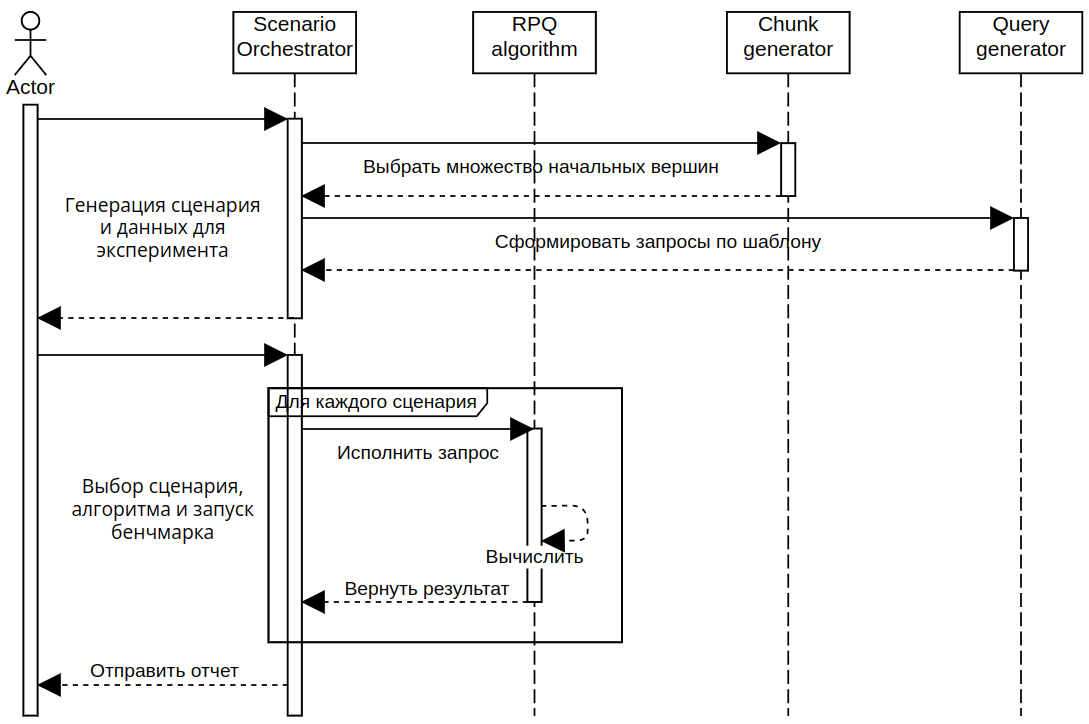
\includegraphics[width=1\linewidth]{pictures/arch.png}
  \caption{Диаграмма последовательностей запуска экспериментов с помощью разработанного инструмента.}
\end{figure}\label{arch}

Перед запуском экспериментов инструмент генерирует данные для соответствующего сценария исполнения. Для этого вызывается \verb|Chunk| \verb|generator|, который выбирает множество начальных вершин графа, на котором будет запущена каждая из реализаций. После чего генерируется множество запросов по определенным заранее шаблонам. Так, \verb|Query| \verb|generator| поддерживает генерацию запросов нескольких видов: в виде регулярного выражения, в виде правил регулярной грамматики и в виде программы на языке Datalog. Создание запросов происходит с помощью конфигурационных файлов, в которых хранятся имена меток на ребрах графа и количество ребер с соответствующей меткой. Благодаря чему удаётся создать запросы с наиболее популярными метками в графе. Шаблоны, по которым формируются запросы выделены в отдельный файл и могут быть изменены. Также, доступен инструмент для подсчета статистики меток в графе, который позволяет создать конфигурационный файл по каждому графу.

Далее, пользователь инициирует выполнение эксперимента на выбранном множестве сценариев. Для каждого из сценариев запускается реализация алгоритма, решающего задачу поиска путей с регулярными ограничениями. После того, как алгоритм закончил исполнение запроса, он возвращает результат в виде числа найденных вершин. В итоге \verb|Scenario orchestrator| сохраняет показатели времени исполнения вычислений в отдельный файл, а также обрабатывает ошибки, которые могли возникнуть во время работы алгоритма. В результате постановки эксперимента отправляется отчет, содержащий информацию о запущенном сценарии, времени исполнения и результате работы алгоритма.


\section{Эксперимент}
% !TeX spellcheck = ru_RU
% !TEX root = vkr.tex

Данный раздел посвящен описанию проводимого экспериментального исследования. В предыдущих главах были представлены основные подходы к исполнению запросов с регулярными ограничениями, а также описан новый алгоритм, основанный на операциях линейной алгебры и поиске в ширину. Сравнение производительности этого алгоритма с реализациями других подходов является основной целью данного исследования.

\subsection{Исследовательские вопросы и метрики}

В качестве основной метрики производительности рассматривается время работы алгоритмов на регулярных запросах.
Цель экспериментального исследования --- ответить на два исследовательских вопроса:

\begin{itemize}
    \item \textbf{RQ1}: Какова производительность разработанного алгоритма по сравнению с существующими аналогами?
    \item \textbf{RQ2}: Как влияет размер множества стартовых вершин на производительность реализации разработанного алгоритма?
\end{itemize}

\subsection{Окружение и конфигурации}

Экспериментальное исследование проводится на сервере под управлением ОС Ubuntu 20.04 со следующими характеристиками: процессор Intel Core i7-6700 CPU, 4 ядра с частотой 3.40 ГГц; объем оперативной памяти 64 Гб.

Для проведения сравнения с аналогом на основе языка Datalog было принято решение использовать язык Souffle~\cite{souffle}, который является одним из диалектов языка Datalog и преодолевает некоторые ограничения классического варианта. Souffle часто используется в задачах языкового анализа и имеет сейчас большую популярность. Установлена версия Souffle 2.4, которая была сконфигурирована с размером слова для примитивного типа 64 бита и запускалась с флагами \verb|-j {число ядер процессора}|, который используется для параллельного исполнения программы, и \verb|--magic-transform=*| для преобразования программы в эквивалентную с потенциально меньшим числом промежуточных вычислений.

Для подхода, основанного на построении индекса, была найдена реализация\footnote{Repository for the prototype code for index RPQ paper: \href{https://github.com/darroyue/Ring-RPQ}{https://github.com/darroyue/Ring-RPQ} (accessed: 20.05.2023)}, находящаяся в свободном доступе, которую автору удалось запустить, однако этот инструмент выдает неверный результат при запуске на сгенерированных по шаблонам запросах, по этой причине он был не включен в сравнительный анализ.

Реализация тензорного алгоритма для нескольких стартовых вершин была взята из репозитория CFPQ\_PyAlgo\footnote{Repository for developing, testing and benchmarking CFPQ algorithms implemented in PyGraphBLAS: \href{https://github.com/FormalLanguageConstrainedPathQuerying/CFPQ_PyAlgo}{https://github.com/FormalLanguageConstrainedPathQuerying/CFPQ\_PyAlgo} (accessed: 20.05.2023)}.

\subsection{Условия эксперимента}

В качестве исходных данных были выбраны графы, собранные по реальным RDF данным и данным социальных сетей. Их характеристики представлены в таблице. В таблице выделено количество вершин и рёбер графа, а также, число уникальных меток, содержащихся на рёбрах. Графы класса RDF расположены в первой части таблицы, графы социальных сетей --- во второй.

\definecolor{lightgray}{gray}{0.9}
\begin{table}[!ht]
    \centering
    \rowcolors{1}{}{lightgray}
    \begin{tabular}{|c|c|c|c|}
        \hline
        Graph      & \#V       & \#E        & \#L \\ \hline \hline
        enzyme     & 48 815    & 86 543     & 14  \\
        eclass     & 239 111   & 360 248    & 10  \\
        go         & 582 929   & 1 437 437  & 47  \\
        geospecies & 450 609   & 2 201 532  & 158 \\
        taxonomy   & 5 728 398 & 14 922 125 & 21  \\
        \hline
        advogato   & 6 541     & 51 127     & 3   \\
        youtube    & 15 088    & 27 257 790 & 5   \\
        \hline
    \end{tabular}
    \caption{Графы.}
\end{table}

Стоит отметить, что графы, собранные по данным социальных сетей являются достаточно плотными в сравнении с графами, построенными по RDF-данным, так как имеют существенно большее число ребер, чем вершин. Это может привести к тому, что во время обхода этих графов будут пройдены более длинные пути, что может сказаться на времени исполнения алгоритмов.

Регулярные запросы к графам были сгенерированы на основе самых популярных шаблонов запросов, собранных в  работе~\cite{related_oneforall}. В запросы входят классические операторы регулярных выражений такие, как конкатенация и перечисление, а также звезда Клини и множество комбинаций этих операторов. Всего отобрано 16 шаблонов, они представлены в таблице~\ref{table:queries}.

\begin{table}[!ht]
    \centering
    \rowcolors{1}{}{lightgray}
    \begin{tabular}{|c|c||c|c|}
        \hline
        Name  & Query                           & Name     & Query                                           \\ \hline \hline
        $q_0$ & $a^*$                           & $q_{8}$  & $a \cdot b$                                     \\
        $q_1$ & $a \cdot b^*$                   & $q_{9}$  & $a \cdot b \cdot c$                             \\
        $q_2$ & $a \cdot b^* \cdot c^*$         & $q_{10}$ & $a \cdot b \cdot c \cdot d$                     \\
        $q_3$ & $a \cdot b^* \cdot c$           & $q_{11}$ & $(a \cdot b)^+~|~(c \cdot d)^+$                 \\
        $q_4$ & $a^* \cdot b^*$                 & $q_{12}$ & $(a \cdot (b \cdot c)^*)^+~|~(d \cdot e)^+$     \\
        $q_5$ & $a \cdot b \cdot c^*$           & $q_{13}$ & $(a \cdot b \cdot (c \cdot d)^*)^+~|~(e~|~f)^*$ \\
        $q_6$ & $(a~|~b~|~c~|~d~|~e)^+$         & $q_{14}$ & $(a~|~b)^+~(c~|~d)^+$                           \\
        $q_7$ & $(a~|~b~|~c~|~d~|~e) \cdot f^*$ & $q_{15}$ & $a \cdot b \cdot (c~|~d~|~e)$                   \\
        \hline
    \end{tabular}
    \caption{Шаблоны запросов.}\label{table:queries}
\end{table}

Для каждого графа отбиралось 5 самых популярных меток, после чего по ним на основе шаблонов генерировалось случайным образом 5 запросов. Важно отметить, что в графе $advogato$ меньше 5 различных меток, по этой причине в сгенерированных для этого графа запросах допускается повторение меток.

В зависимости от числа вершин, на которых запускаются регулярные запросы, их можно разделить на несколько видов:
\begin{itemize}
    \item Single-source запросы, для которых алгоритм запускается от одной исходной вершины.
    \item Multiple-source запросы запускаются от определенного изначально множества вершин в графе.
    \item All-pairs запросы запускаются от множества всех вершин графа.
\end{itemize}

Для выбора множества начальных вершин было решено создавать случайные выборки из нужного числа вершин. Так, для single-source запросов создавалось множество из 100 начальных вершин, для каждой из которых запускался запрос. Для multiple-source запросов создавалась выборка из 2, 5, 10, 100, 1000, 10000 случайных вершин для каждого графа, на которой запускались запросы. При этом финальными считались все вершины графа. Скрипты для создания запросов и генерации вершин доступны в репозитории\footnote{Benchmark suite for RPQ evaluation:~\href{https://github.com/bahbyega/paths-benchmark}{https://github.com/bahbyega/paths-benchmark}~(accessed: 20.05.2023)}.

\subsection{Результаты сравнения алгоритмов}
\textbf{RQ1}: Какова производительность разработанного алгоритма по сравнению с существующими аналогами?

На рисунках 3--4 представлены результаты эксперимента по сравнению производительности алгоритмов на графах, построенных по RDF данным. Введены следующие обозначения: алгоритм, основанный на поиске в ширину, обозначен MSBFS, алгоритм, основанный на тензорном произведении --- Tensor, решение, основанное на Datalog и реализованное с помощью диалекта Souffle --- Datalog. Для всех шаблонов в виде гистограмм представлено среднее арифметическое значение времени исполнения алгоритмов с отклонением от среднего на соответствующем запросе.

Прежде всего эксперимент был поставлен на графах наименьшего размера --- \textit{enzyme} и \textit{eclass} для случая single-source запросов, который представлен в первой колонке. Результаты показывают, что реализации алгоритмов в терминах матричных операций в среднем на порядок быстрее реализации на Datalog. В частности, алгоритм на основе тензорного произведения работает более чем в 10 раз быстрее аналога на Datalog, алгоритм MSBFS --- в среднем в 100 раз быстрее. Важно отметить, что программы для аналога на Datalog генерировались по соответствующим представлениям регулярных ограничений в виде грамматик. Реализовать каждый из запросов для конкретного графа можно эффективнее, используя дополнительные средства языка Souffle, что могло повлиять на показатели времени, представленные на рисунках.

Далее, три реализаций запускались на multiple-source запросах. Результаты для наибольшего из множеств начальных вершин (10000 вершин) представлены на рисунках 3--4 во второй колонке. На множестве из 10000 стартовых вершин Tensor и Datalog показывают близкую производительность, проигрывая MSBFS. При этом показатели времени исполнения тензорным алгоритмом имеют более высокое отклонение от среднего значения. Это может объясняться тем, что конкретный шаблон представлен несколькими запросами с метками, расположенными в разном порядке. Из-за чего результат исполнения запроса может сильно отличаться по количеству достижимых вершин. Так, для шаблонов $q_6$, $q_8$, $q_9$, $q_{10}$ большое значение имеет порядок, в котором расставлены метки в шаблоне, потому что в них отсутствует оператор звезды Клини.

После чего проводился эксперимент на графе \textit{go}. Из него видно, что производительность MSBFS оказалась незначительно хуже алгоритма, основанного на тензорном произведении. Это может быть объяснено структурой графа \textit{go}. Он имеет большое число ребер с одной и той же меткой, которая чаще всего встречалась в запросах, что повлияло на количество шагов алгоритма MSBFS.

По экспериментам на графах \textit{geospecies} и \textit{taxonomy} также можно выделить лучшую производительность MSBFS и Tensor относительно Datalog. Однако тензорный алгоритм демонстрирует выбросы на некоторых запросах, когда запрос запускается на множестве из 10000 вершин. Кроме того, важно отметить, что производительность алгоритмов зависит от сложности запроса. Так, запросы $q_7$ и $q_{13}$, содержащие в себе большее количество меток и операторов, чем остальные запросы, исполняются в среднем дольше остальных.

% !TeX spellcheck = ru_RU
% !TEX root = vkr.tex

\newcolumntype{C}{ >{\centering\arraybackslash} m{4cm} }
\newcommand\myvert[1]{\rotatebox[origin=c]{90}{#1}}
\newcommand\myvertcell[1]{\multirowcell{5}{\myvert{#1}}}
\newcommand\myvertcelll[1]{\multirowcell{4}{\myvert{#1}}}
\newcommand\myvertcellN[2]{\multirowcell{#1}{\myvert{#2}}}

\afterpage{
    \clearpage
    \thispagestyle{empty}
    \begin{landscape}
        \centering
        \begin{figure}
            \begin{tabular}{cc}
                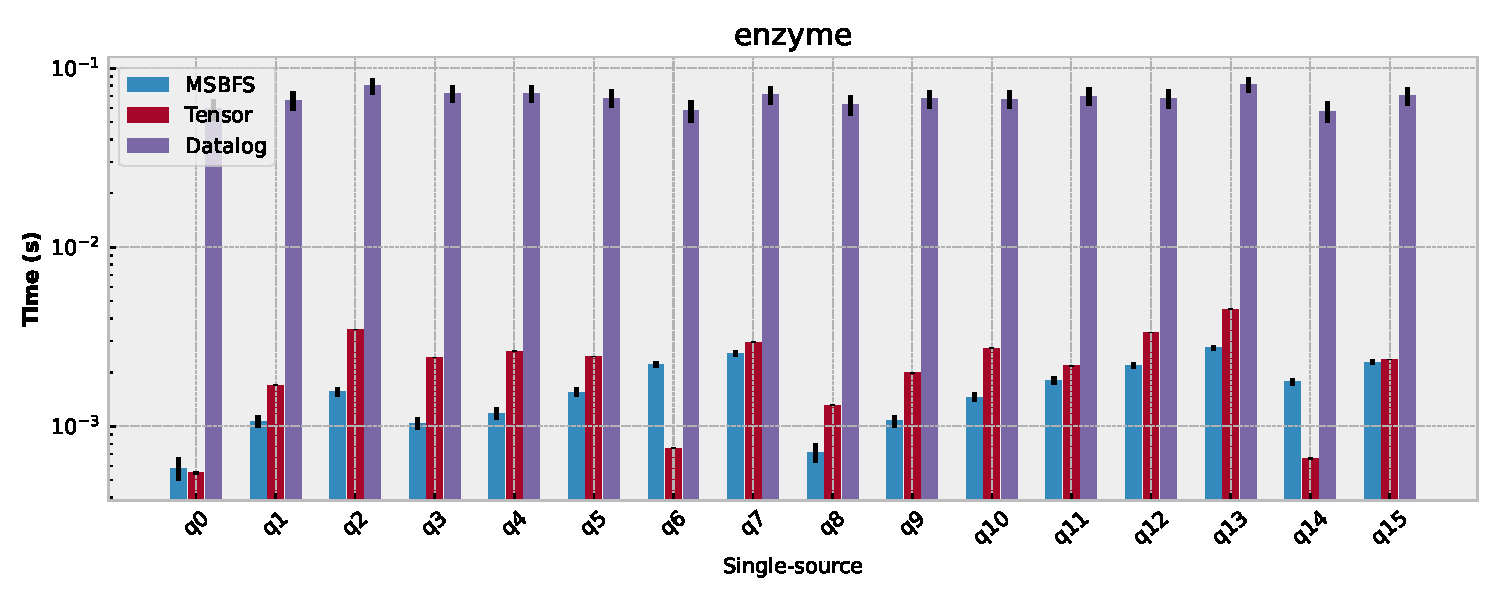
\includegraphics[width=120mm]{pictures/enzyme_ss.pdf} & 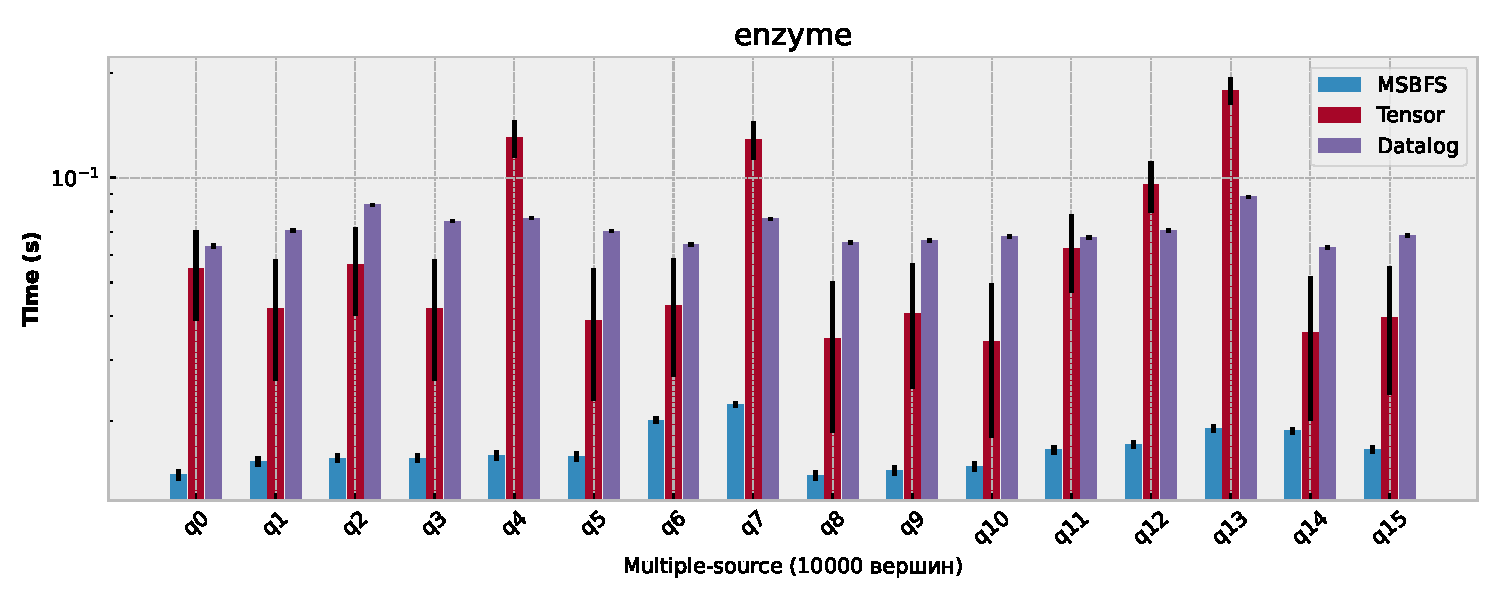
\includegraphics[width=120mm]{pictures/enzyme_ms10000.pdf} \\
                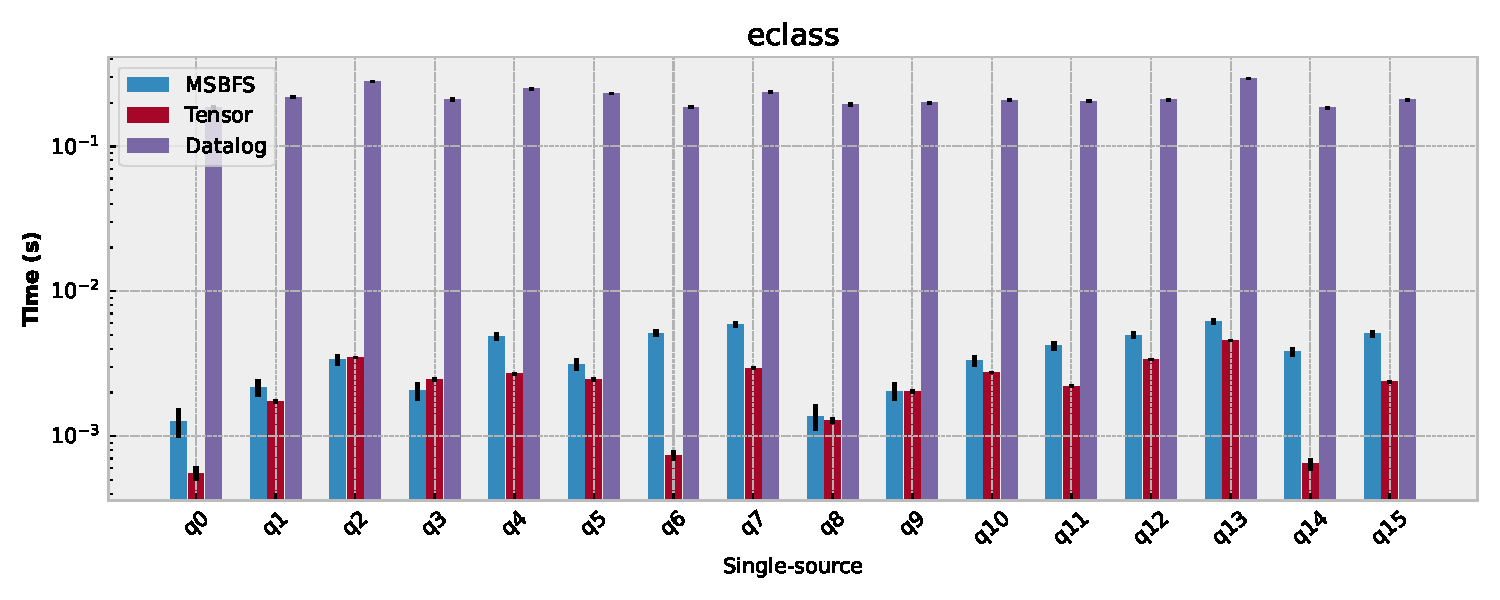
\includegraphics[width=120mm]{pictures/eclass_ss.pdf} & 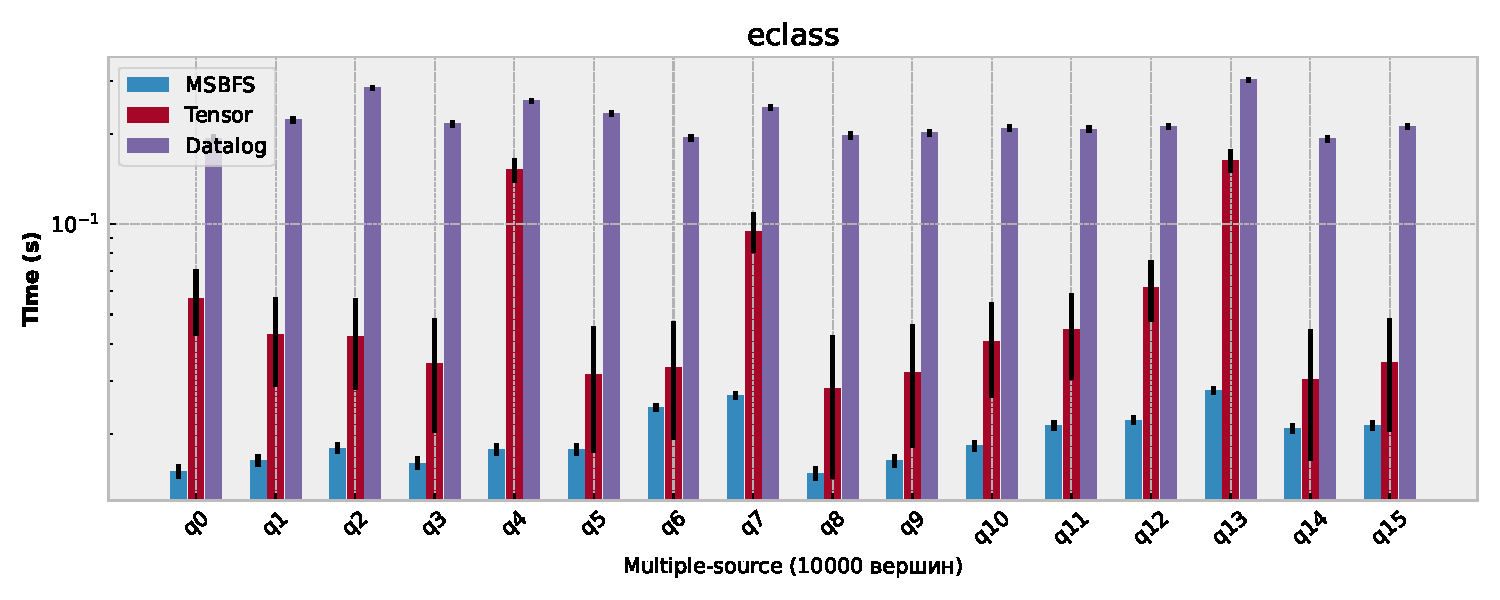
\includegraphics[width=120mm]{pictures/eclass_ms10000.pdf} \\
                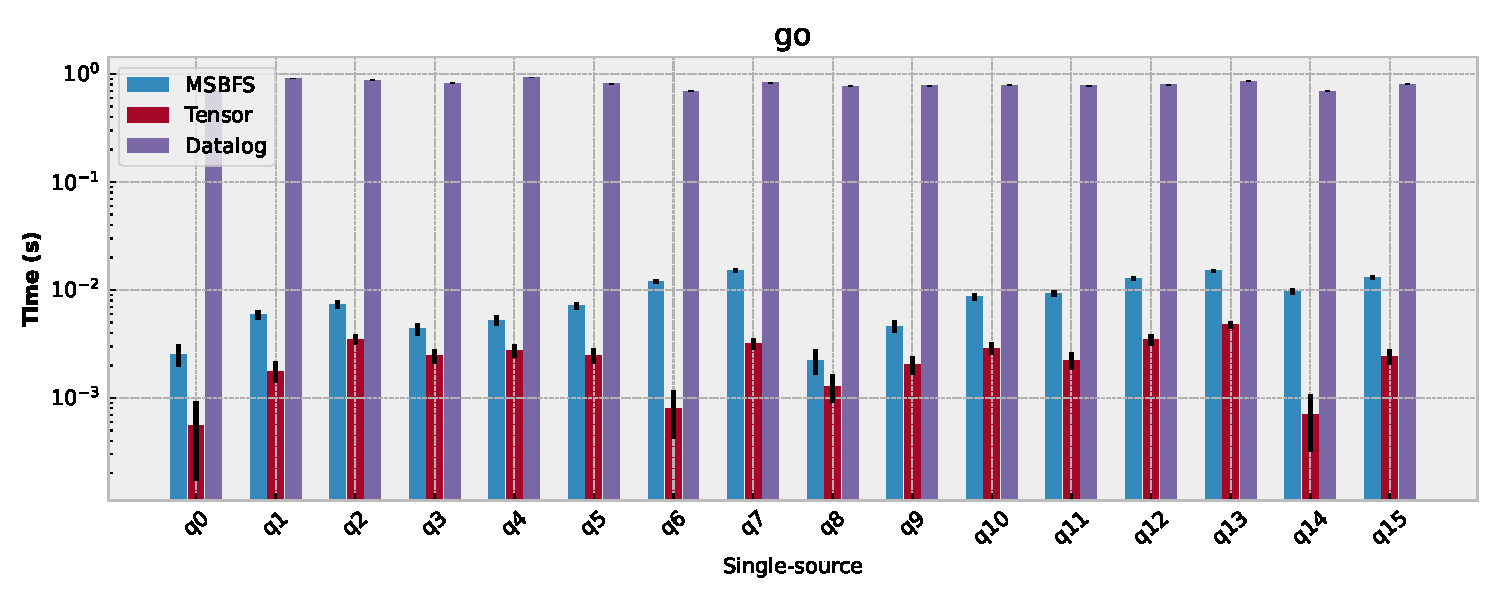
\includegraphics[width=120mm]{pictures/go_ss.pdf}     & 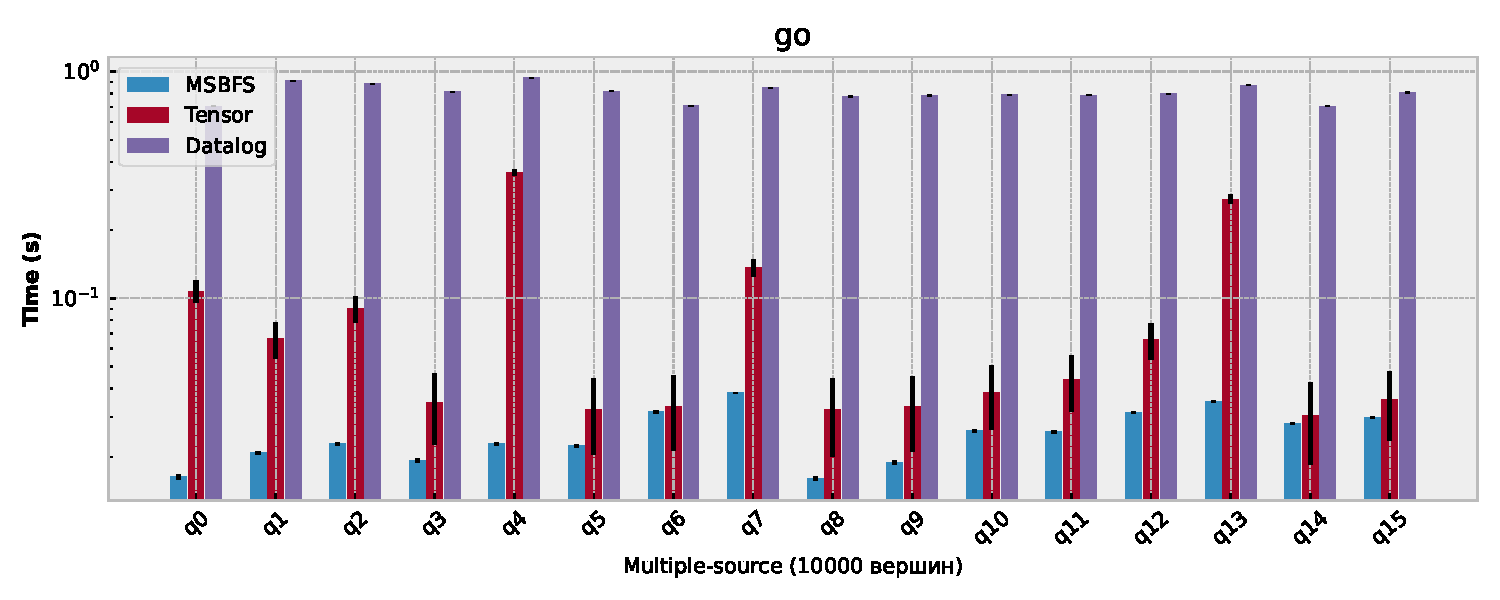
\includegraphics[width=120mm]{pictures/go_ms10000.pdf}     \\
            \end{tabular}
            \caption{Результаты эксперимента на наборе RDF-данных для single-source и multiple-source (10000 вершин) запросов.}
        \end{figure}
    \end{landscape}
    \clearpage
}

% !TeX spellcheck = ru_RU
% !TEX root = vkr.tex

\afterpage{
    \clearpage
    \thispagestyle{empty}
    \begin{landscape}
        \centering
        \begin{figure}
            \begin{tabular}{cc}
                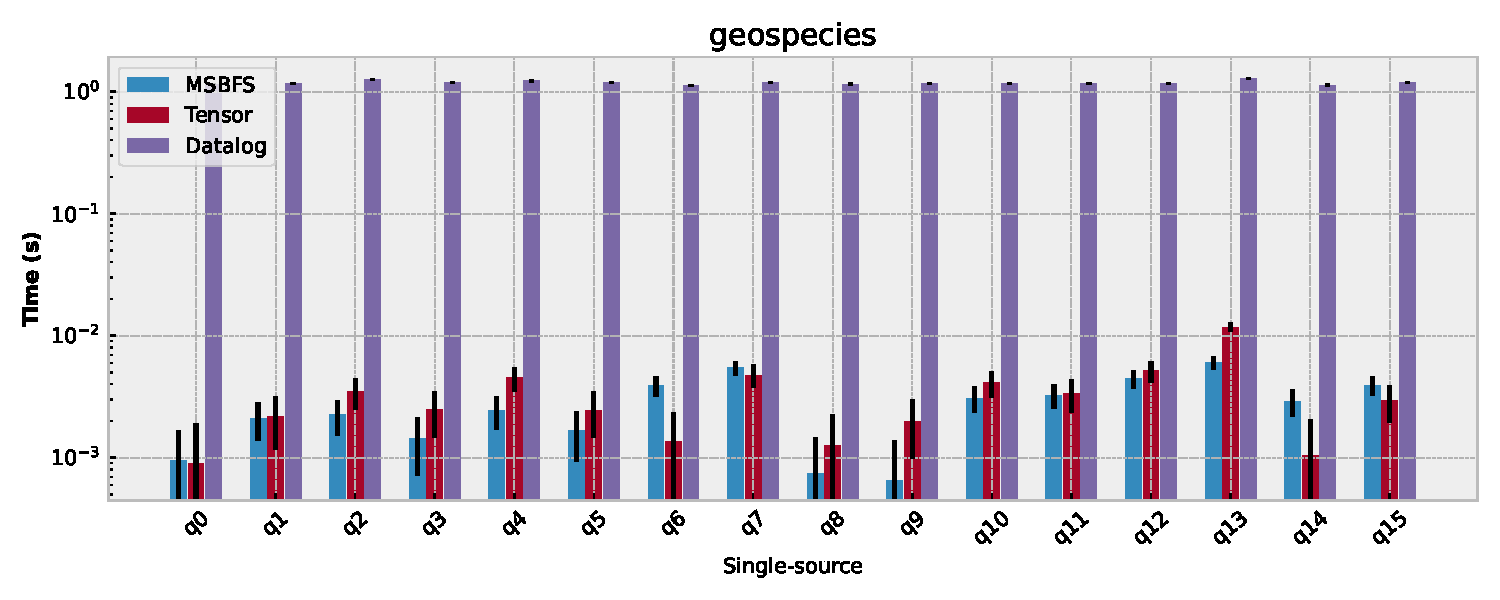
\includegraphics[width=120mm]{pictures/geospecies_ss.pdf} & 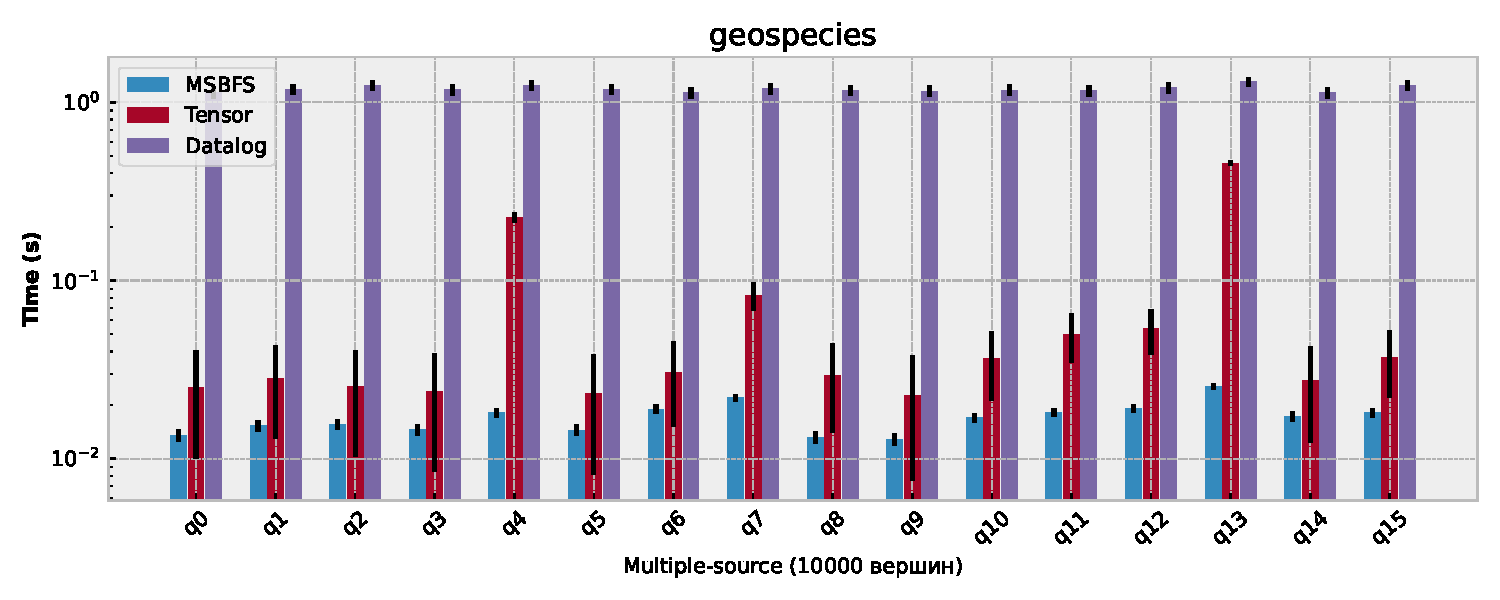
\includegraphics[width=120mm]{pictures/geospecies_ms10000.pdf} \\
                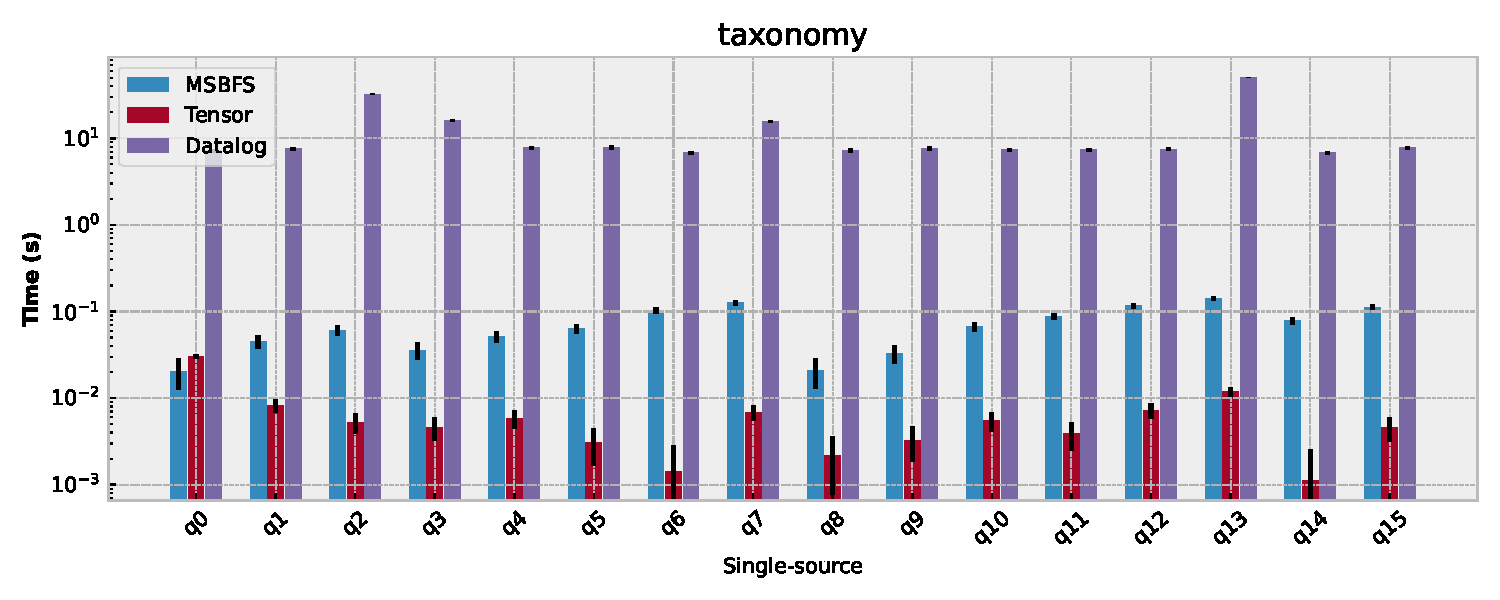
\includegraphics[width=120mm]{pictures/taxonomy_ss.pdf}   & 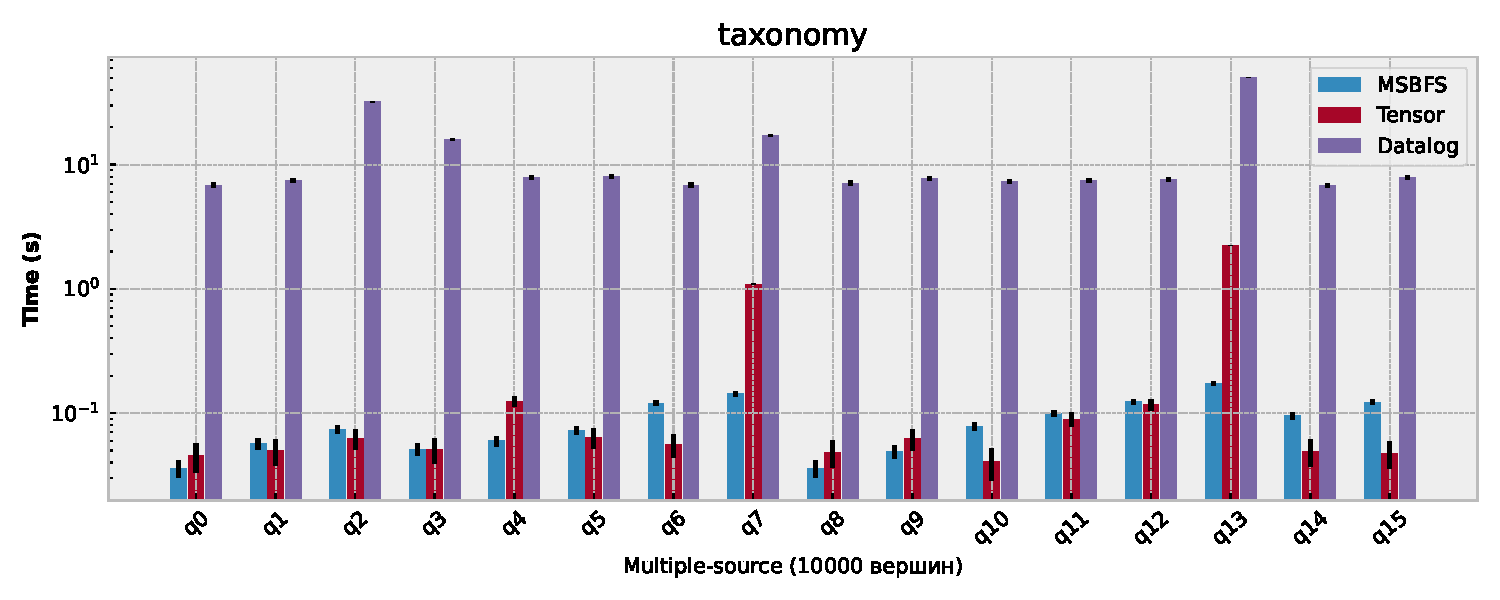
\includegraphics[width=120mm]{pictures/taxonomy_ms10000.pdf}   \\
            \end{tabular}
            \caption{Результаты эксперимента на наборе RDF-данных для single-source и multiple-source (10000 вершин) запросов.}
        \end{figure}
    \end{landscape}
    \clearpage
}


\textbf{RQ2}: Как влияет размер множества стартовых вершин на производительность реализации разработанного алгоритма?

\begin{figure}
    \begin{tabular}{cc}
        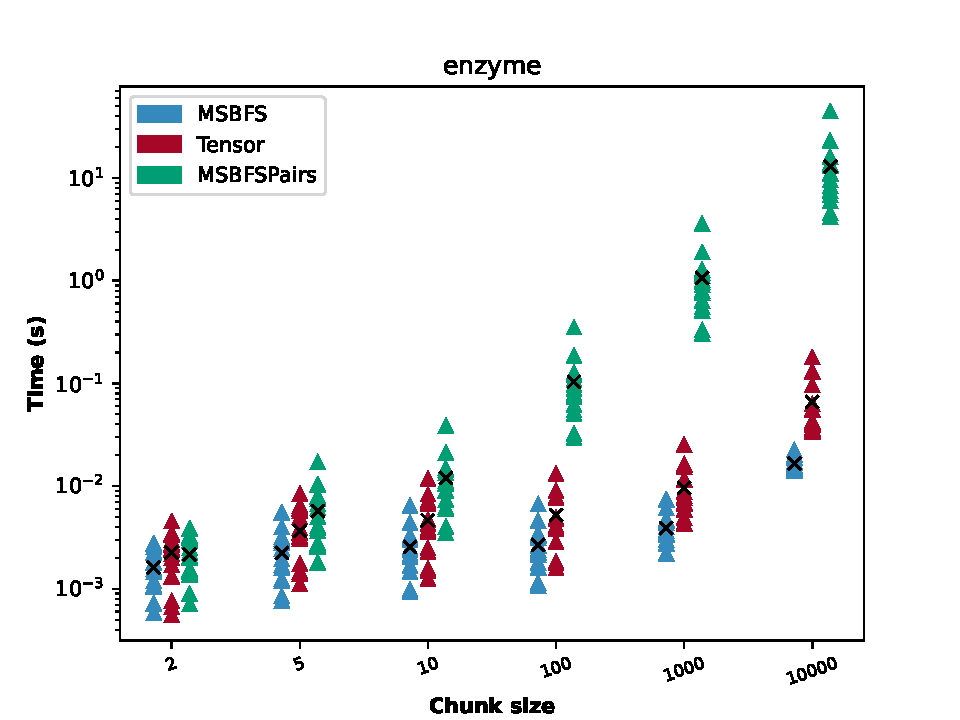
\includegraphics[width=85mm]{pictures/chunks-enzyme.pdf}     & 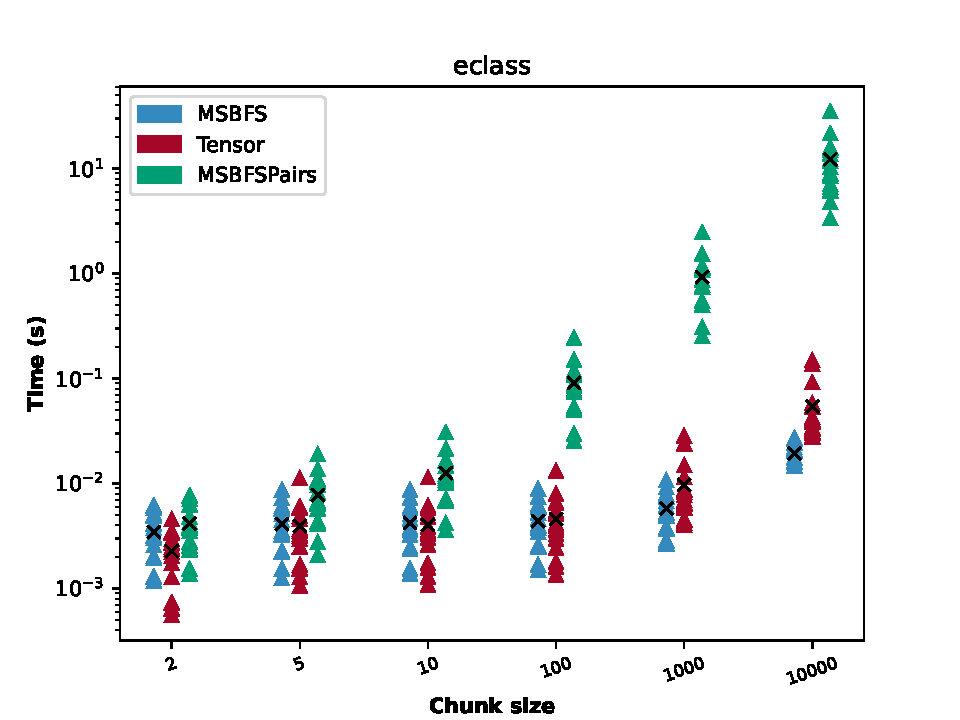
\includegraphics[width=85mm]{pictures/chunks-eclass.pdf}   \\
        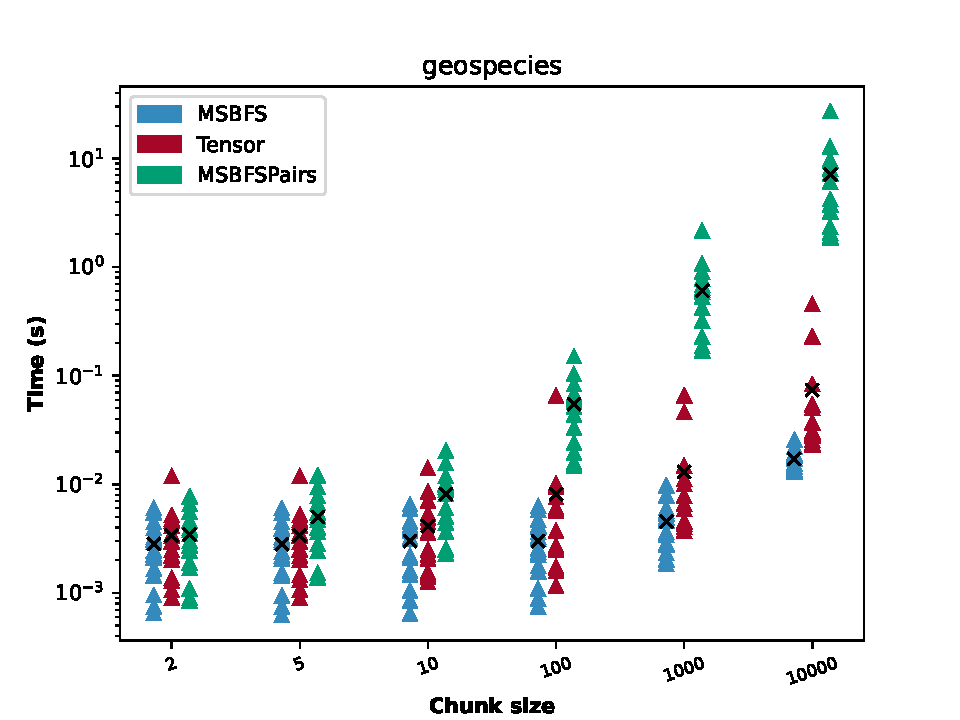
\includegraphics[width=85mm]{pictures/chunks-geospecies.pdf} & 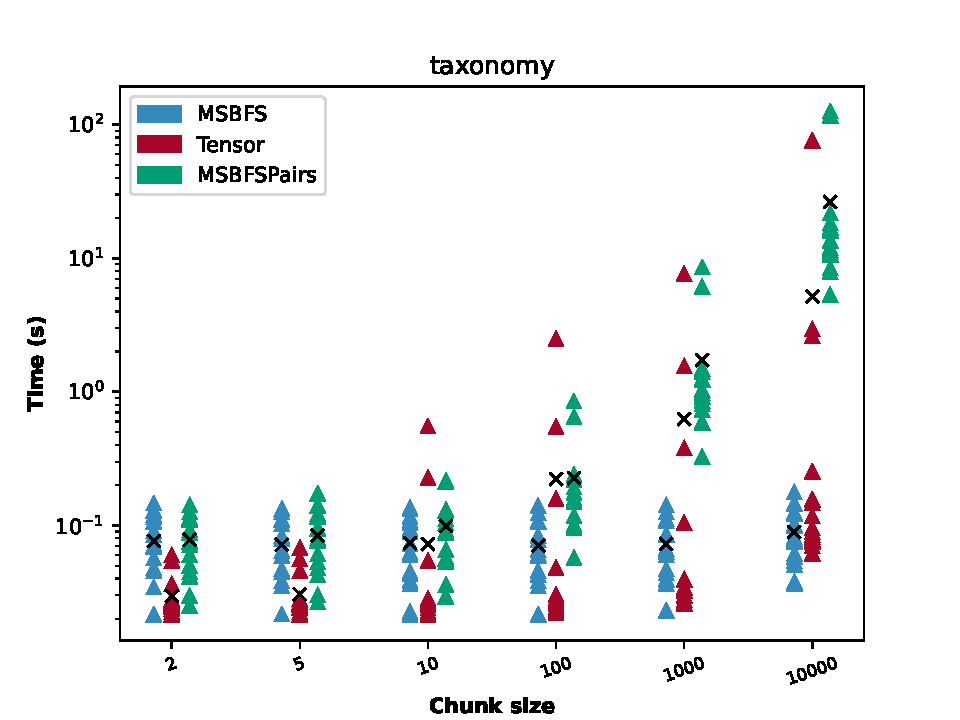
\includegraphics[width=85mm]{pictures/chunks-taxonomy.pdf} \\
        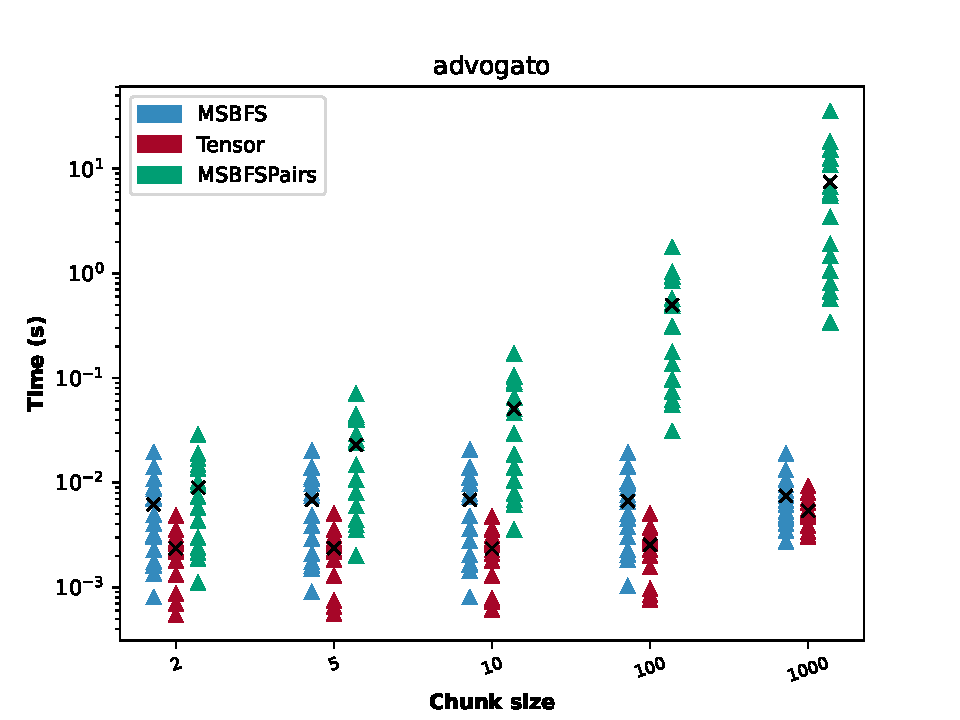
\includegraphics[width=85mm]{pictures/chunks-advogato.pdf}   & 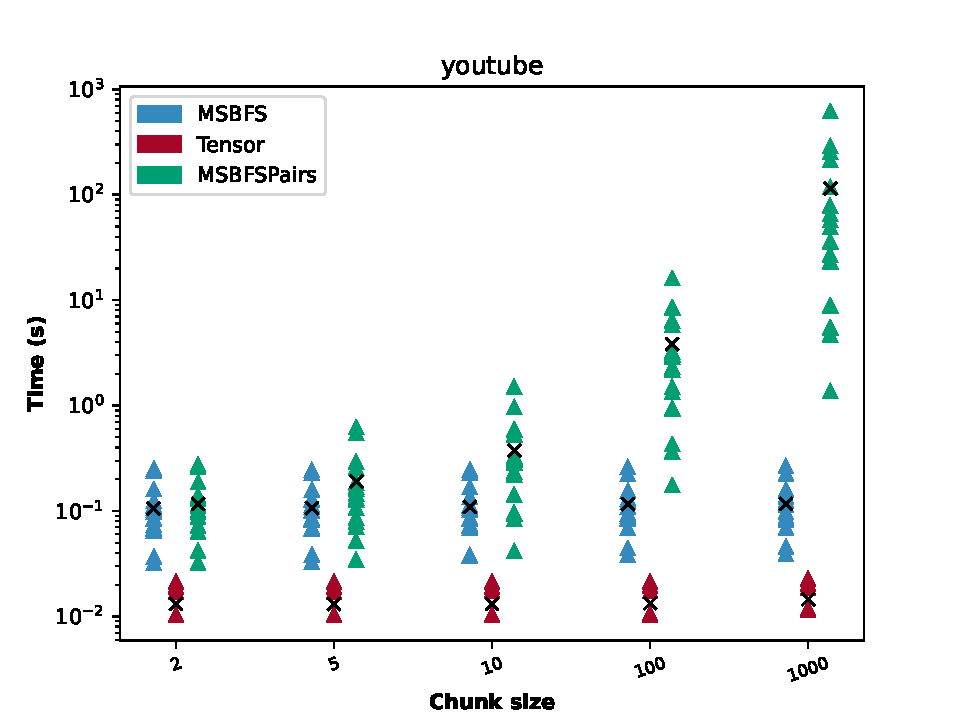
\includegraphics[width=85mm]{pictures/chunks-youtube.pdf}  \\
    \end{tabular}
    \caption{Результаты эксперимента с multiple-source запросами для разных выборок стартовых вершин.}
\end{figure}\label{chunks_bfs_vs_tensor}

Результаты эксперимента по анализу производительности алгоритма для различного числа стартовых вершин представлены на рисунке~\ref{chunks_bfs_vs_tensor}. На нем изображена зависимость времени исполнения запроса от числа стартовых вершин в графе для алгоритмов MSBFS и Tensor. Для выявления зависимости числа стартовых вершин ко времени исполнения была взята еще одна реализация MSBFS, обозначенная MSBFSPairs, которая, в отличие от MSBFS, находит не множество достижимых вершин, а пары начальная--конечная вершина. Основной особенностью этой реализации является то, что инициализация матриц стартовыми вершинами увеличивает размер перемножаемых матриц в $n$ раз, где $n$ --- число стартовых вершин. Это позволяет запомнить от какой стартовой вершины была достигнута каждая из вершин в конечном множестве достижимых. Отмечено время исполнения каждого из запросов, а также выделено среднее время их исполнения. Результаты показывают, что с ростом числа стартовых вершин время работы алгоритма MSBFS меняется несущественно. Это может объясняться тем, что инициализация матриц стартовыми вершинами в его реализации не влияет на размер перемножаемых матриц, что не создает дополнительных расходов во время работы алгоритма, в то время как алгоритмы Tensor и MSBFSPairs страдают от существенного снижения производительности при росте числа стартовых вершин.

Также, на основе этого рисунка можно сделать вывод о том, что время исполнения запроса зависит не только от размера графа, но и от его структуры и разреженности. Так, по анализу данных социальных сетей можно сделать вывод о том, что алгоритм на основе тензорного произведения демонстрирует лучшую производительность для более плотных графов, таких как \textit{advogato} и \textit{youtube}. Именно эти графы имеют наименьшее число различных меток, граф \textit{youtube} также имеет наибольшее число ребер среди всех графов датасета при существенно меньшем числе вершин. Это приводит к тому, что алгоритму, основанному на поиске в ширину, приходится выполнять больше шагов во время обхода графа, так как на этих графах с каждым шагом алгоритма более вероятно увеличение фронта обхода.

Результаты анализа экспериментального исследования позволяют заключить, что реализация алгоритма, основанного на поиске в ширину, показывает приемлемую производительность и во многих случаях работает быстрее, чем реализации аналогов. Более того, реализация алгоритма MSBFS для нахождения всего множества достижимых вершин показывает несущественное ухудшение производительности с ростом числа стартовых вершин. В то же время, реализация алгоритма MSBFSPairs, результатом которого является множество пар начальная--конечная вершина, показала худшие временные характеристики. Более того, заметным является падение производительности обоих реализаций MSBFS на графах социальных сетей, что может быть исследовано в дальнейшем на более широком наборе данных.


\pagebreak

\section*{Заключение}
% !TeX spellcheck = ru_RU
% !TEX root = vkr.tex

При проведении данной работы были достигнуты следующие результаты. 

\begin{itemize}
    \item Проведен обзор и выбрано два доступных аналога для проведения сравнительного анализа, а именно, тензорный алгоритм и алгоритм на основе языка Datalog. Последний является принятым базовым инструментом.
    \item Собран набор данных, состоящий из графов и регулярных запросов, для проведения экспериментального исследования. В него вошли графы собранные по RDF-данным и данным социальных сетей, а также множество популярных запросов.
    \item Спроектирован инструмент, который позволяет автоматизировать проведение экспериментов, поддерживает генерацию данных для запуска запросов на графах, получение множества начальных вершин и запуск различных типов запросов\footnote{Benchmark suite for RPQ evaluation:~\href{https://github.com/bahbyega/paths-benchmark}{https://github.com/bahbyega/paths-benchmark} (accessed: 20.05.2023)}.
    \item Проведено экспериментальное исследование алгоритма и сравнение с аналогами. В ходе анализа было выявлено, что подход к реализации алгоритма поиска путей с ограничениями в виде регулярных языков на основе поиска в ширину является жизнеспособным и показывает приемлемые результаты на реальных данных. 
    Более того, на RDF-данных алгоритм показывает кратный рост производительности относительно аналога, реализованного на Datalog, а также работает в среднем быстрее алгоритма, основанного на тензорном произведении. Тем не менее, анализ зависимости времени исполнения запроса к числу стартовых вершин выявил проблемы реализации алгоритма MSBFS для решения задачи достижимости от каждой стартовой вершины, что может быть исследовано в дальнейшей работе. 
    \end{itemize}

В дальнейшем работа может быть развита в следующих направлениях.
\begin{itemize}
    \item Расширение набора данных, на котором исследуется алгоритм. В него можно включить искусственно сгенерированные графы с определенными особенностями структуры, а также реальные графы из других прикладных областей.
    \item Интегрирование алгоритма с графовой базой данных, а также с языком запросов к графовой базе данных. Это позволит провести еще более полноценное сравнение алгоритма с аналогами, в которые можно будет включить системы графовых баз данных. 
\end{itemize}
\noindent 


\setmonofont[Mapping=tex-text]{CMU Typewriter Text}
\bibliographystyle{ugost2008ls}
\bibliography{vkr}

\end{document}
